\documentclass[a4paper,11pt]{article}
\usepackage{a4wide}
\usepackage{fullpage}
\usepackage[utf8x]{inputenc}
%\usepackage[slovene]{babel}
%\selectlanguage{slovene}
\usepackage[toc,page]{appendix}
\usepackage[pdftex]{graphicx} 
\usepackage{amsfonts}
\usepackage{amsmath}
\usepackage{setspace}
\usepackage{color}
\definecolor{light-gray}{gray}{0.95}
\usepackage{listings} 
\usepackage{hyperref}
\renewcommand{\baselinestretch}{1.2} 
\renewcommand{\appendixpagename}{Priloge}

\lstset{ 
language=Python,
basicstyle=\footnotesize,
basicstyle=\ttfamily\footnotesize\setstretch{1},
backgroundcolor=\color{light-gray},
}

\title{Topological data analysis \\ Homework 2}
\author{Sara Bizjak (27202020)}
\date{\today}

\begin{document}

\maketitle

%%%%%%%%%%%%%%%%%%%%%%%%%%%%%%%%%%%%%%%%%%%%%%%%%%%%%%%%%%%%%%%%%%%%%%%%%%%%%%%%%%%%%%%%%%%%%%%%%%%%%%%%%%%%%%%%%%%%%%%%%%%%%%%%%%%%%%%%%%%%%%%%%%%%%%%%%%%%%%%%

\section{Theoretical problems}
\subsection{Triangulations}

%%%%%%%%%%%%%%%%%%%%%%%%%%%%%%%%%%%%%%%%%%%%%%%%%%%%%%%%%%%%%%%%%%%%%%%%%%%%%%%%
\noindent
a) Show that they are at most $ 2^{ \frac{n(n-1)}{2} } $ triangulations of S.
\\
A triangulation is a decomposition of S into triangles, such that:

\begin{itemize}
    \item no triangle is degenerate,
    \item interiors of the triangles are disjoint,
    \item the intersection of any two triangles is a common edge, a common vertex or empty.
\end{itemize}

\noindent
In other words, a triangulation is a maximal crossing-free geometric graph on a point set S, or a subgraph of general plane graph (and also of maximal general plane graph).
\\
A maximal general plane graph $G$ (with vertices $S$) is a graph with all possible connections between vertices and has $(n - 1) + (n - 2) + \ldots + 3 + 2 + 1$ connections, shortly written as $ \frac{n(n - 1)}{2} $.
If we take a look at subgraphs of $G$, we can quickly conclude that there are $ 2 ^ { \frac{n(n-1)}{2}} $ possible subgraphs, since with every connection we can choose to add it to the subgraph or not.
\\
Since a triangulation is a subgraph of $G$ and the number of all subsets of such graph is $ 2 ^ { \frac{n(n-1)}{2}} $, we can conclude that there are at most $ 2 ^ { \frac{n(n-1)}{2}} $ triangulations of set $S$.
\\

%%%%%%%%%%%%%%%%%%%%%%%%%%%%%%%%%%%%%%%%%%%%%%%%%%%%%%%%%%%%%%%%%%%%%%%%%%%%%%%%

\noindent
b) Constructing a set $S$ such that all possible triangulations of $S$ have a point of degree $n−1$.
\\
The degree of a point in a triangulation $T$ is the number of edges in $T$, incident to that point.
\\
Therefore, in a set $S$ has to be a point that is connected to all other points, for example, the red point on a picture has always a degree $ n - 1$. 

\begin{figure}[ht!] 
    \centering
    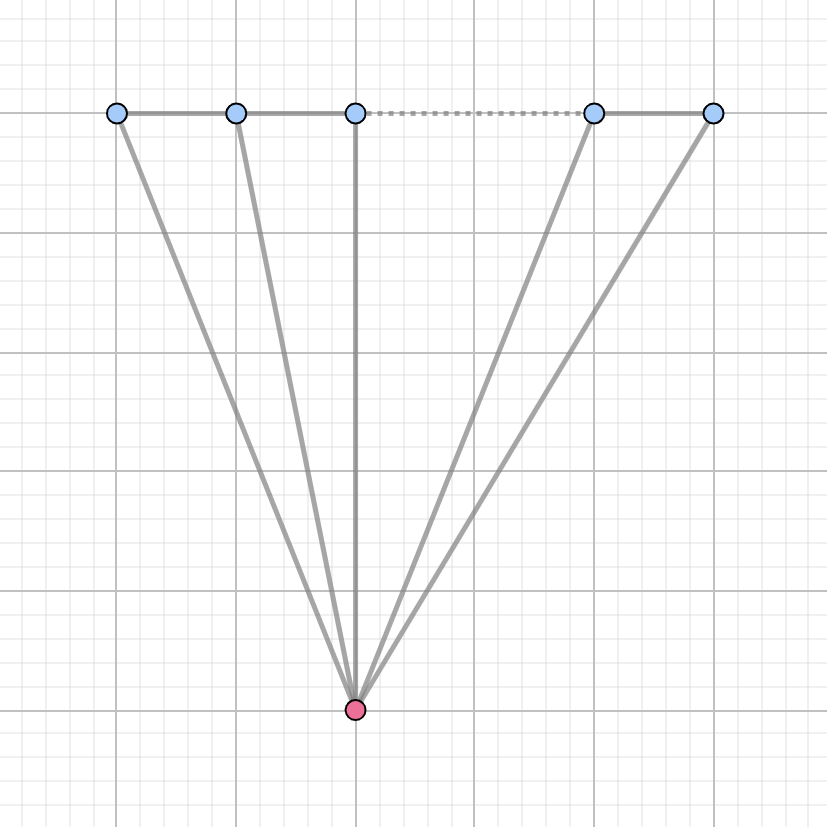
\includegraphics[width=60mm]{1b.png}
    \caption{Construction of set $S$.}
\end{figure}

%%%%%%%%%%%%%%%%%%%%%%%%%%%%%%%%%%%%%%%%%%%%%%%%%%%%%%%%%%%%%%%%%%%%%%%%%%%%%%%%

\newpage
\noindent
c) Show that any triangulation $T$ of $S$ has a point of degree $5$ or less using the fact that 
if not all points in $S$ are collinear, then any triangulation $T$ of $S$ has at most $3n−3$ edges ($|E| \leq 3n - 3$).
\\
Proof with contradiction. Assume every point in $T$ has a degree 6 or more, so $\text{deg}(v) \geq 6$ for all $v \in V$.
\\
Since every connection has 2 edges, it follows that $2|E| = |V| = \sum_{v \in V} \text{deg}(v)$.
\\
By using the fact that all points in $T$ has a degree al least 6, we can calculate that
$$ 2|E| = |V| = \sum_{v \in V} \text{deg}(v) \geq \sum_{v \in V} 6 = 6n $$
and it follows that $ |E| \geq 3n $.
From the proposition we know that $|E| \leq 3n - 3$ and if we combine both equations, we get 
$$ 3n \leq |E| \leq 3n - 3 \Rightarrow 0 \leq 3 $$
which is in contradiction, hence the proposal is true.

%%%%%%%%%%%%%%%%%%%%%%%%%%%%%%%%%%%%%%%%%%%%%%%%%%%%%%%%%%%%%%%%%%%%%%%%%%%%%%%%%%%%%%%%%%%%%%%%%%%%%%%%%%%%%%%%%%%%%%%%%%%%%%%%%%%%%%%%%%%%%%%%%%%%%%%%%%%%%%%%

\subsection{Vietoris-Rips Complex and Čech Complex}
Let $S = \{ (0,0),(2,0),(1,0.5),(1,1.5) \} \in \mathbb{R}^2$, where $A = (0,0),$ $B = (2,0),$ $C = (1,0.5),$ $D = (1,1.5)$.
\\

%%%%%%%%%%%%%%%%%%%%%%%%%%%%%%%%%%%%%%%%%%%%%%%%%%%%%%%%%%%%%%%%%%%%%%%%%%%%%%%%

\noindent
a) Building the Vietoris-Rips complex Rips$(S, 2\epsilon)$ and the Čech complex Cech$(S, \epsilon)$ for $ \ \epsilon = 0.8$.
\\
In the Vietoris-Rips complex $\text{Rips}(S, 2\epsilon)$ two vertices are connected by an edge if and only if the distance between them is less or equal to $2 \epsilon$.
To check that, we draw closed balls of radius $\epsilon$ centered in points from given set $S$.
We construct Rips$(S, 2\epsilon)^{(1)}$ and the next thing we want to do is to find all possible complete subgraphs.
\\
For $2 \epsilon = 1.6$ (or $\epsilon = 0.8$) we get Rips$(S, 1.6)^{(1)} = \{A, B, C, D, AC, BC, CD\}$. There are no simplices of dimension 2 or higher in Rips$(S, 1.6)^{(1)}$, 
so Rips$(S, 1.6)$ $=$ Rips$(S, 1.6)^{(1)}$ and dim(Rips$(S, 1.6)) = 1$ with Euler characteristic $\chi = 4 - 3 = 1$.

\begin{figure}[ht!]
    \begin{minipage}{0.5\textwidth}
        \centering
        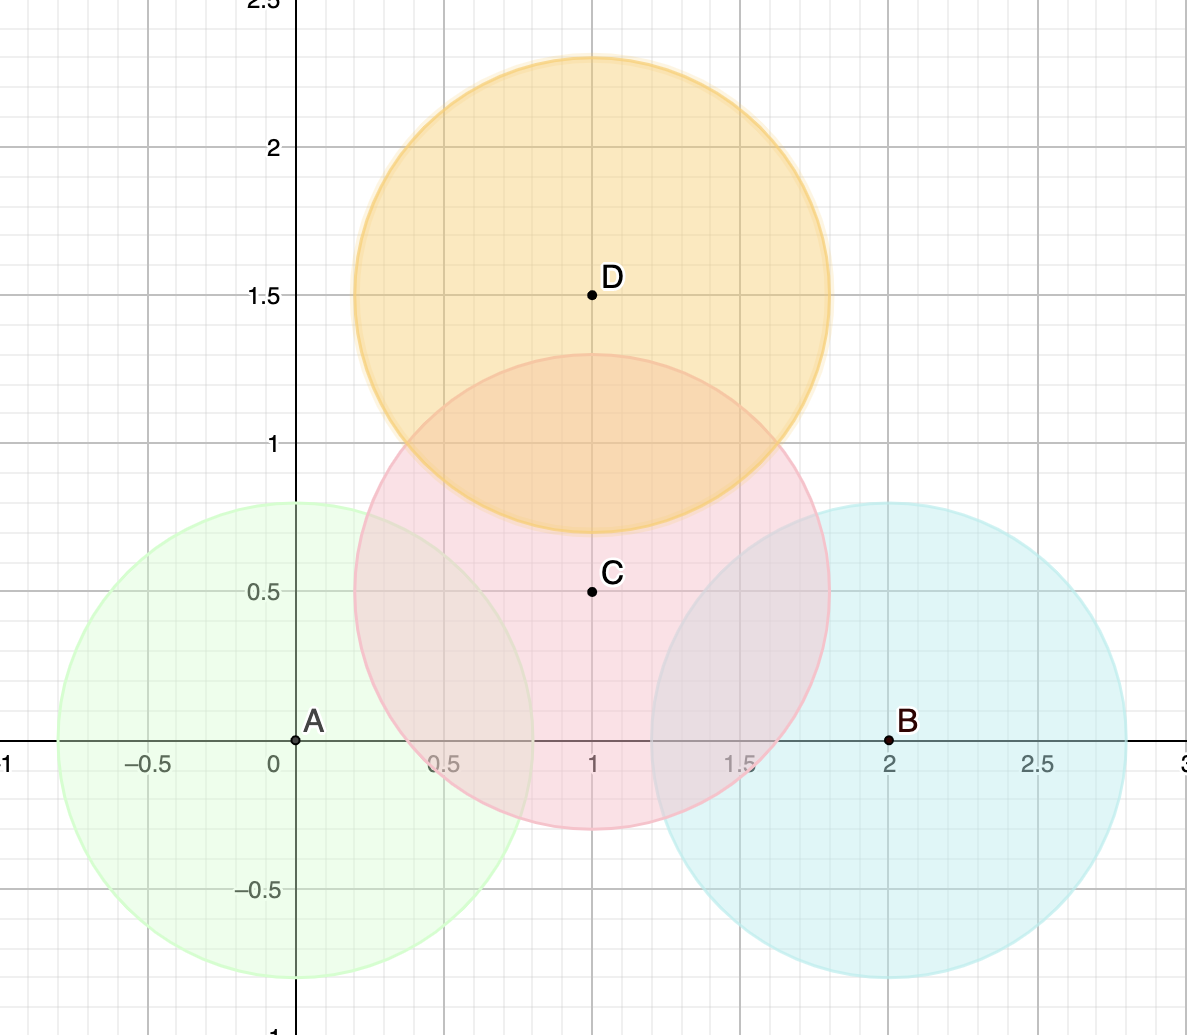
\includegraphics[width=60mm]{r08.png}
        \caption{$\epsilon = 0.8$.}
    \end{minipage}\hfill
    \begin{minipage}{0.5\textwidth}
        \centering
        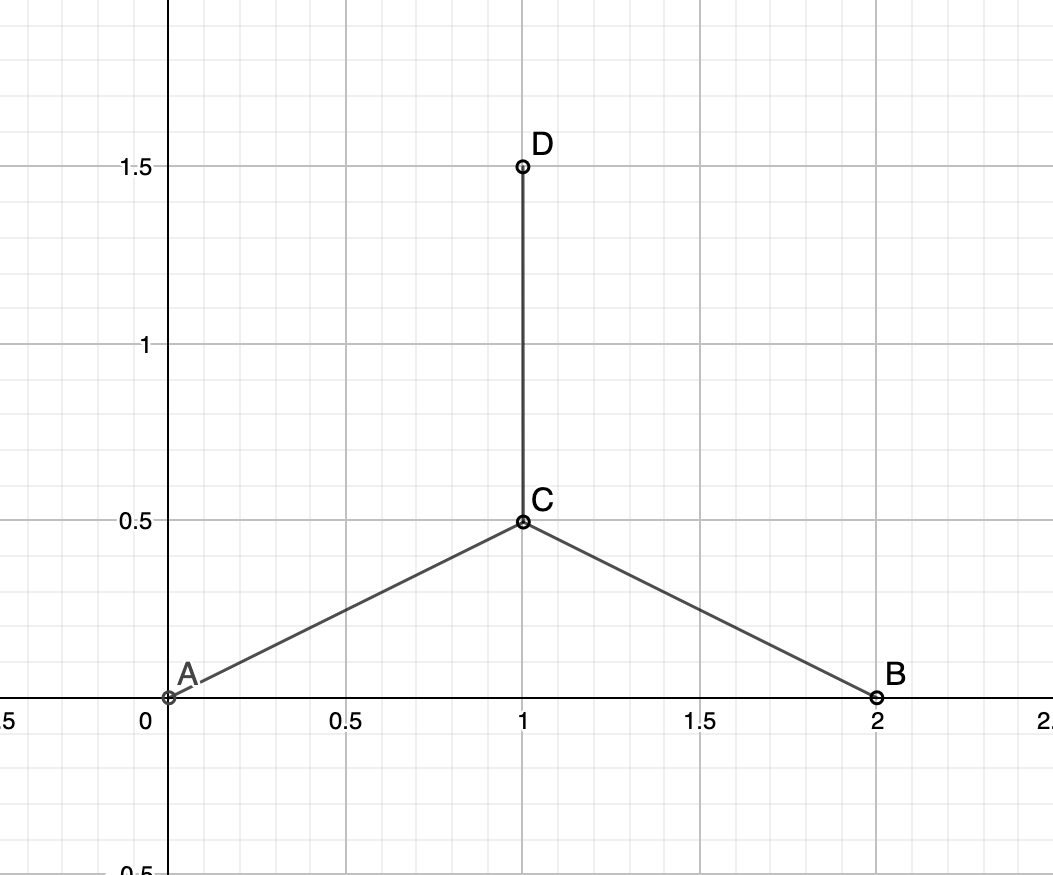
\includegraphics[width=60mm]{08povezave.png}
        \caption{$\epsilon = 0.8$.}
    \end{minipage}\hfill
\end{figure}
\noindent
The Čech complex Cech$(S, \epsilon)$ is the nerve of the cover of $S$ with balls of radius $\epsilon$, so we can reuse the images.
It is true that Cech$(S, \epsilon)^{(1)}$ = Rips$(S, 2 \epsilon)^{(1)}$ and Cech$(S, \epsilon)$ $\subset$ Rips$(S, 2 \epsilon)$.
\\
So the Vietoris-Rips and Čech complexes are the same in this case.
\\
\\

%%%%%%%%%%%%%%%%%%%%%%%%%%%%%%%%%%%%%%%%%%%%%%%%%%%%%%%%%%%%%%%%%%%%%%%%%%%%%%%%

\noindent
b) Building the Vietoris-Rips complex Rips$(S, 2\epsilon)$ and the Čech complex Cech$(S, \epsilon)$ for $ \ \epsilon = 1$.
\\
For $2 \epsilon = 2$ (or $\epsilon = 1$) we get Rips$(S, 2)^{(1)} = \{A, B, C, D, AB, AC, AD, BC, BD, CD\}$. We also have three copies of $K_3$ $(ABC, ACD, BCD)$ and one of $K_4$ (ABCD), so 
Rips$(S, 2)$ = Rips$(S, 2)^{(1)}$ $\cup \ \{ ABC, ACD, BCD\} \cup \{ ABCD\}$ and dim(Rips$(S, 2)) = 3$ with Euler characteristic $\chi = 4 - 6 + 3 -1 = 0$.

\begin{figure}[ht!]
    \begin{minipage}{0.5\textwidth}
        \centering
        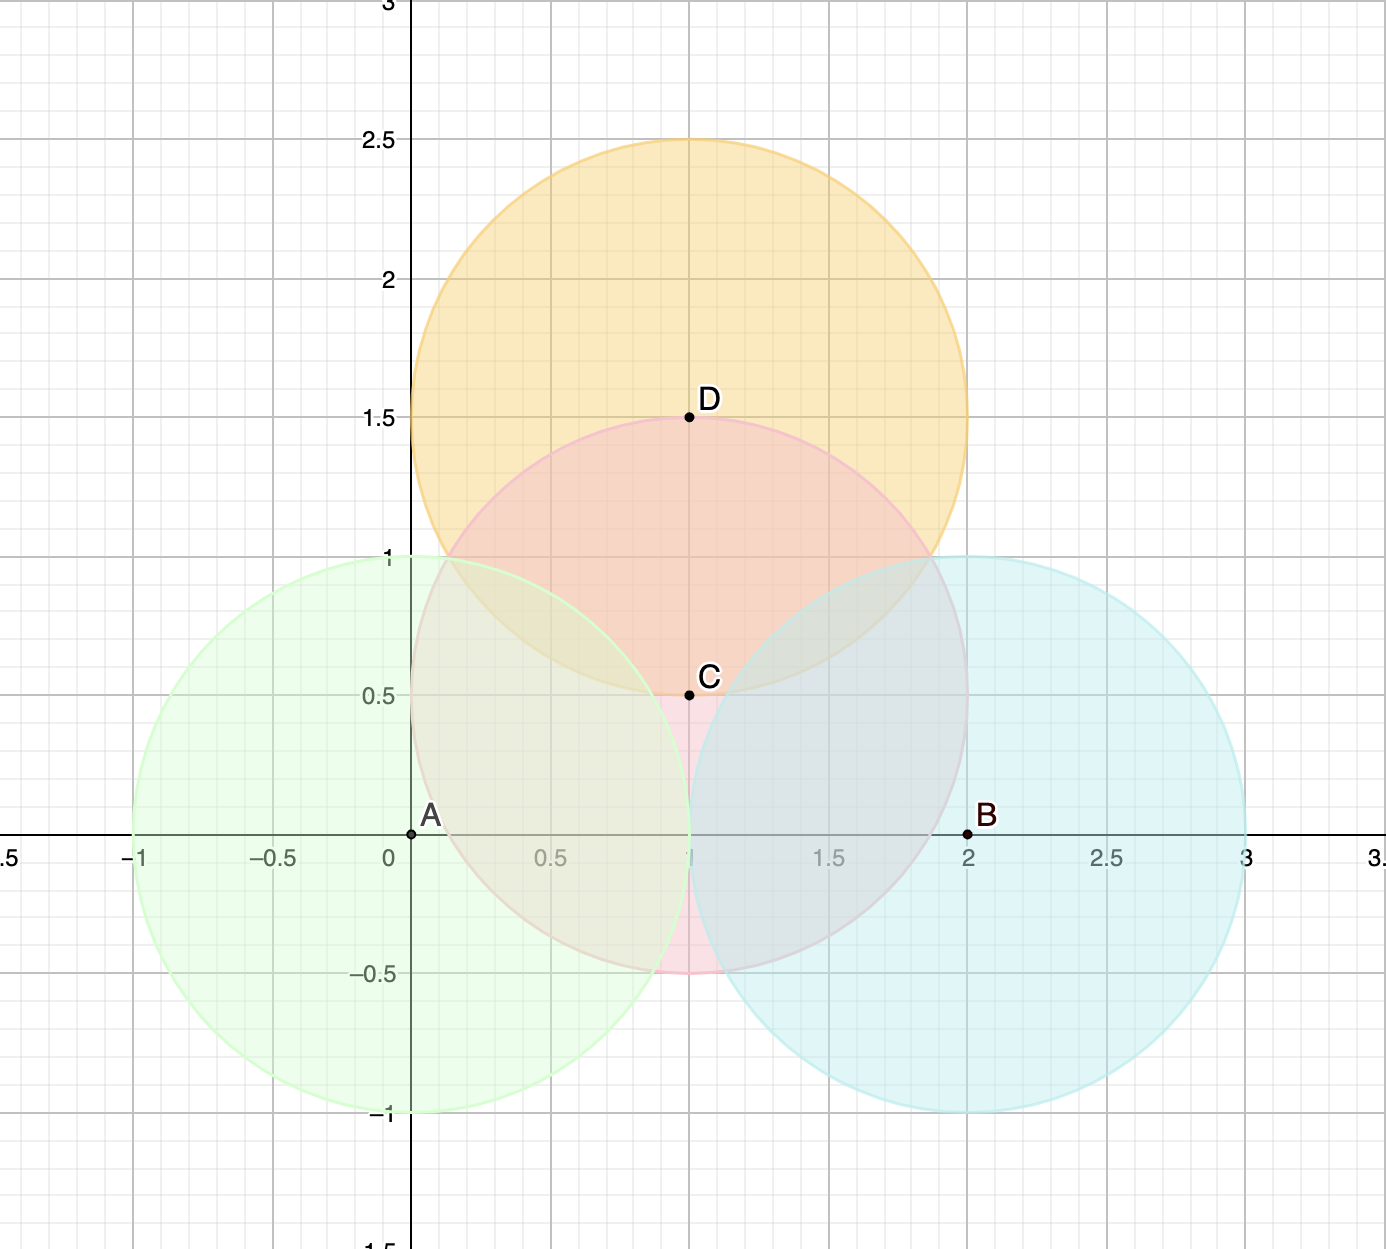
\includegraphics[width=60mm]{r1.png}
        \caption{$\epsilon = 1$.}
    \end{minipage}\hfill
    \begin{minipage}{0.5\textwidth}
        \centering
        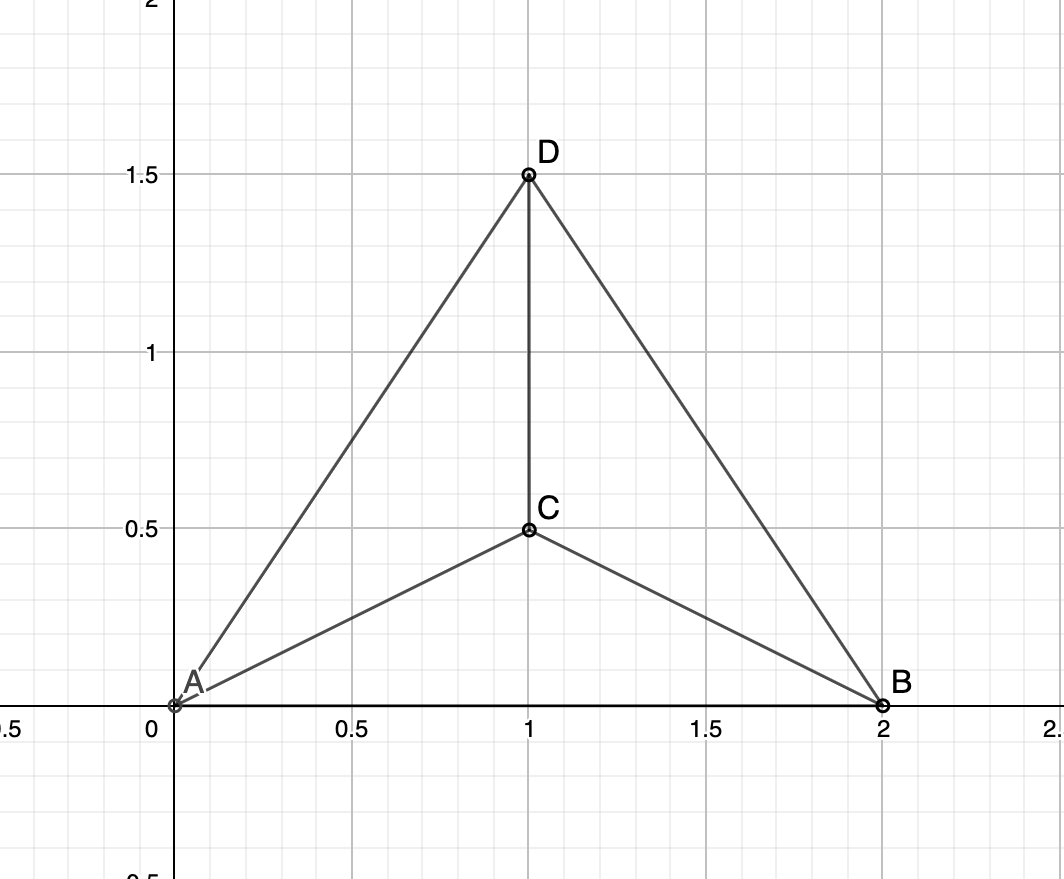
\includegraphics[width=60mm]{1povezave.png}
        \caption{$\epsilon = 1$.}
    \end{minipage}\hfill
\end{figure}
\noindent
Since all of three circles centered in points $A, B, C$, points $A, C, D$ and points $B, C, D$ have a non-empty triple intersection (all four don't), all three $2-$simplices from Rips$(S, 2)$ are also contained in Cech$(S, 1)$.
Cech$(S, 1)$ = $\{A, B, C, D, AB, AC, AD, BC, BD, CD, ABC, ACD, BCD\}$ and dim(Cech$(S, 1)) = 2$ with Euler characteristic $\chi = 4 - 6 + 3 = 1$.

%%%%%%%%%%%%%%%%%%%%%%%%%%%%%%%%%%%%%%%%%%%%%%%%%%%%%%%%%%%%%%%%%%%%%%%%%%%%%%%%%%%%%%%%%%%%%%%%%%%%%%%%%%%%%%%%%%%%%%%%%%%%%%%%%%%%%%%%%%%%%%%%%%%%%%%%%%%%%%%%

\subsection{Voronoi diagram}
Finding a configuration of $n$ points ($n >3$) in the plane such that their Voronoi diagram will have a cell with $n−1$ vertices.
\\
The Voronoi diagram is a decomposition of $\mathbb{R}^2$ into Voronoi regions, where the Voronoi region $V_a$ of $a \in S$ is $V_a = \{ x \in \mathbb{R}^2 ; \ d(x, a) \leq d(x, a') \ \forall a' \in S \}$.
\\
Such configuration of $n$ points is $n - 1$ points on the circle and one point in the middle of that circle.

\begin{figure}[ht!]
    \centering
    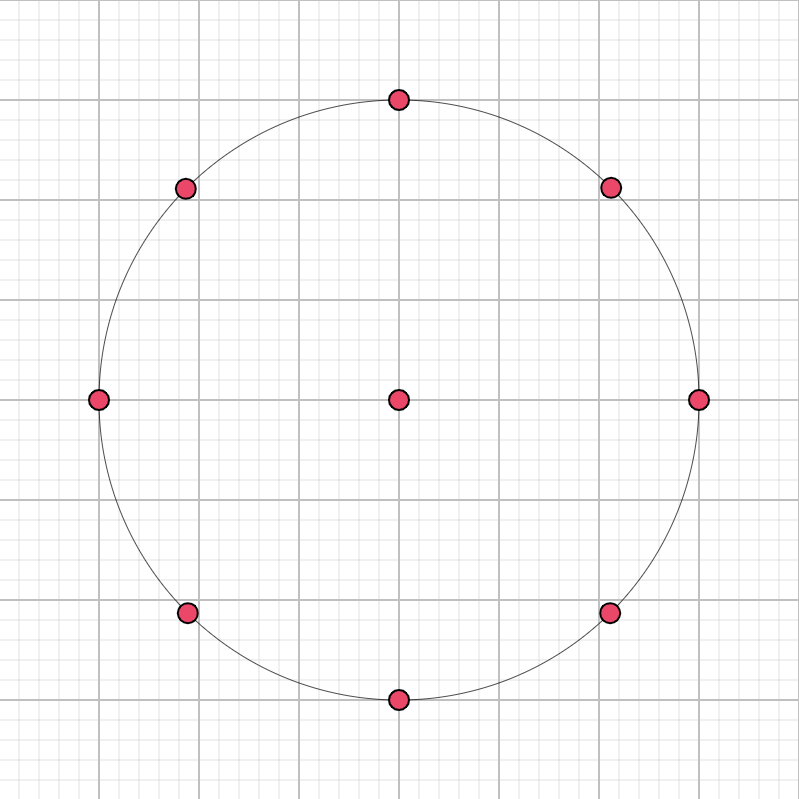
\includegraphics[width=50mm]{1_3.png}
    \caption{Example for $n = 9$.}
\end{figure}

%%%%%%%%%%%%%%%%%%%%%%%%%%%%%%%%%%%%%%%%%%%%%%%%%%%%%%%%%%%%%%%%%%%%%%%%%%%%%%%%%%%%%%%%%%%%%%%%%%%%%%%%%%%%%%%%%%%%%%%%%%%%%%%%%%%%%%%%%%%%%%%%%%%%%%%%%%%%%%%%

\subsection{Chessboard Complex}
The chess board complex of a $m \times n$ chessboard is a simplicial complex $\Delta_{m \times n}$. The vertices of $\Delta_{m \times n}$ correspond to the squares of the chessboard. Simplices of $\Delta_{m \times n}$ correspond to non-taking placements of rooks (ie. placements where no two rooks are in the same columnor in the same row).
\\

%%%%%%%%%%%%%%%%%%%%%%%%%%%%%%%%%%%%%%%%%%%%%%%%%%%%%%%%%%%%%%%%%%%%%%%%%%%%%%%%

\noindent
a) Showing that the chessboard complex $\Delta_{3 \times 2}$ is homeomorphic to the circle $S^1$.  (Showing that the simplicial complex you obtain is a 1-dimensional connected manifold with no boundary.)
\\
If we follow the hint, we can read the proof of the picture. This is a 1-dimensional complex with a connected circular path with no boundary (all the vertices and edges are interior -- two connections from one vertex). 

\begin{figure}[ht!]
    \centering
    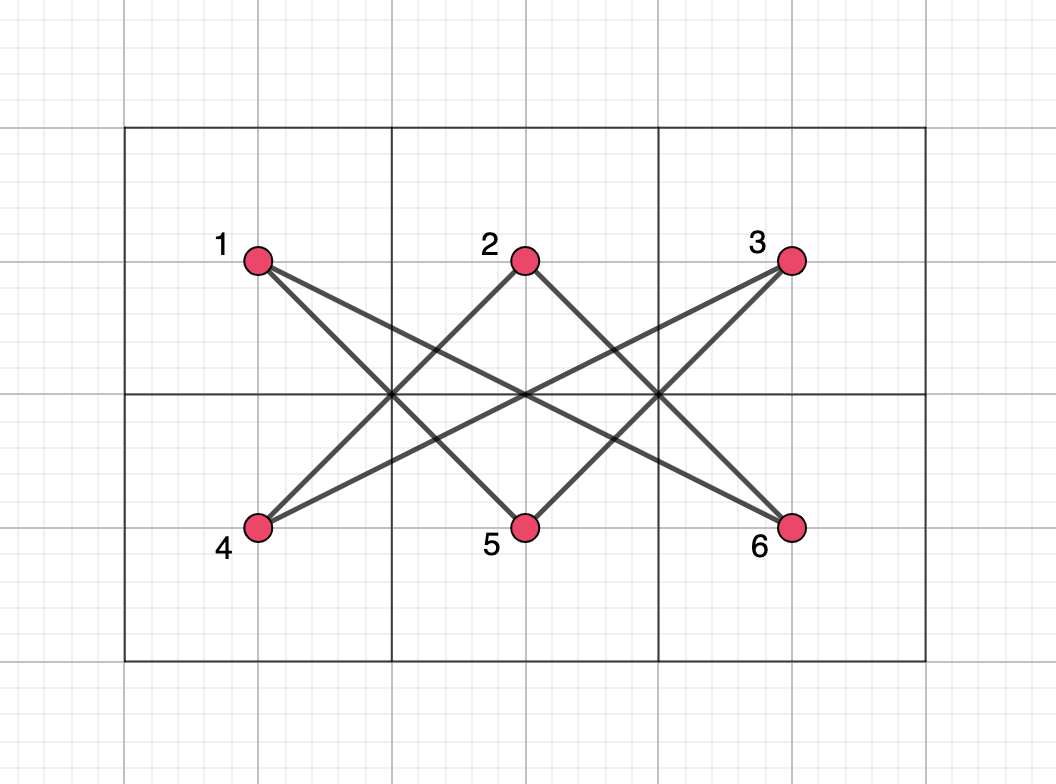
\includegraphics[width=80mm]{1_4_a.png}
    \caption{$\Delta_{3 \times 2}$.}
\end{figure}
\noindent 
$\Rightarrow$ Chessboard complex $\Delta_{3 \times 2}$ is homeomorphic to the circle $S^1$.
\\
\\

%%%%%%%%%%%%%%%%%%%%%%%%%%%%%%%%%%%%%%%%%%%%%%%%%%%%%%%%%%%%%%%%%%%%%%%%%%%%%%%%

\noindent
b) Showing that the chessboard complex $\Delta_{4 \times 3}$ is homeomorphic to a torus $S^1 \times S^1$. (Showing that the complex we obtain is an orientable connected 2-dimensional manifold without boundary with Euler characteristic 0.)
\\
Following the hint:
\\
If we take a look at the picture we can see that every point is connected to exactly 6 other points. That 6 points represent the 1-dim complex from task a),
for which we know it is homeomorphic to the circle $S^1$. When we connect those 6 points to every point, we get 2-dimensional complex.
\\
This 2-dimensional complex has a connected circular path with no boundary, since each point has an even number of connections.
The path is orientable -- for a selected a point we can choose any other point and determin the orientation of surrounding of that point. We can also determin the orientation the other way around. In other words, we can "travel" around our manifold in any direction and are able to determin the orientation.
This manifold has exactly two different possible orientations, so it is connected and oriantable.
\\
Euler characteristic is $\chi = 12 - \frac{12 \cdot 6}{2} + \frac{2 \cdot \frac{6 \cdot 12}{2}}{3} = 12 - 36 + 24 = 0$.

\begin{figure}[ht!]
    \centering
    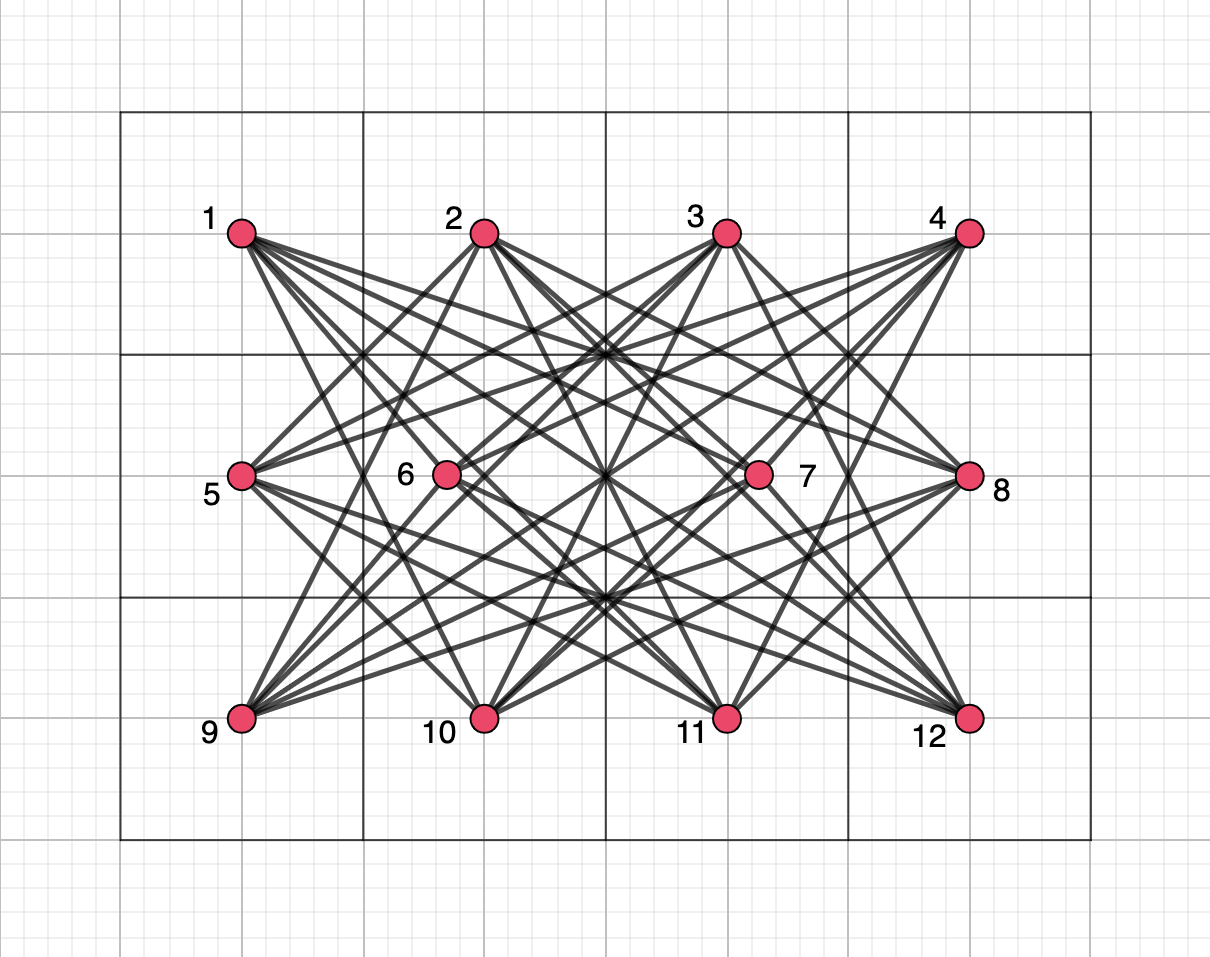
\includegraphics[width=80mm]{1_4_b.png}
    \caption{$\Delta_{3 \times 2}$.}
\end{figure}
\noindent
$\Rightarrow$ Chessboard complex $\Delta_{4 \times 3}$ is homeomorphic to a torus $S^1 \times S^1$.
\\

%%%%%%%%%%%%%%%%%%%%%%%%%%%%%%%%%%%%%%%%%%%%%%%%%%%%%%%%%%%%%%%%%%%%%%%%%%%%%%%%

\noindent
c) Showing that the chessboard complex $\Delta_{n \times (n - 1)}$ is a manifold for all $n$.
\\
From taskst a) and b) we know that $\Delta_{3 \times 2}$ is a 1-dim manifold and $\Delta_{4 \times 3}$ is a 2-dim manifold.
With induction we would like to show that $\Delta_{n \times (n - 1)}$ is a $(n - 2)$-dim manifold assuming that $\Delta_{(n - 1) \times (n - 2)}$ is a $(n - 3)$-dim manifold.
\\
If we look at the pictures for complexes $\Delta_{3 \times 2}$ and $\Delta_{4 \times 3}$ we can see that we added a row and a column with relevant connections
to make a $\Delta_{4 \times 3}$ from $\Delta_{3 \times 2}$ manifold.
So by adding new points and connections, we combined 1-dim manifold into 2-dim manifold.
\\
Approaching the same idea we can combine $(n - 3)$-dim manifold $\Delta_{(n - 1) \times (n - 2)}$ and get $\Delta_{n \times (n - 1)}$ manifold (by adding $n + n - 2$ points to $\Delta_{(n - 1) \times (n - 2)}$ manifold -- a row and a column), which is one dimension higher, so it is a $(n - 2)$-dim manifold.
\\
$\Rightarrow$ Chessboard complex $\Delta_{n \times (n - 1)}$ is a $(n - 2)$-dim manifold for all $n$.
\\

%%%%%%%%%%%%%%%%%%%%%%%%%%%%%%%%%%%%%%%%%%%%%%%%%%%%%%%%%%%%%%%%%%%%%%%%%%%%%%%%%%%%%%%%%%%%%%%%%%%%%%%%%%%%%%%%%%%%%%%%%%%%%%%%%%%%%%%%%%%%%%%%%%%%%%%%%%%%%%%%

\subsection{Vietoris-Rips Complex and Čech Complex in $d_{\infty}$ metric}
Proving that if we define the Vietoris-Rips and the Čech Complex using $d_{\infty}$ metric instead of $d_2$, then the complexes we obtain for any given$\ \epsilon$ are the same, ie. $\text{C}_{\epsilon} = \text{VR}_{2 \epsilon}$.
\\
Metric $d_{\infty}$, also known as Chebyshev metric, is a metric defined on a vector space, where the distance between two vectors is the greatest of their differences along any coordinate dimensions.
$$ d_{\infty}(x, y) := \text{max}_i ( | x_i - y_i | ) \ , \ (x_i, y_i) \in \mathbb{R}^d$$
First recall Vietoris-Rips and Cech complex definitions.

$$\text{VR}_{2 \epsilon}(S) := \{ T \subseteq S ~|~ \text{diam}(T) \leq \epsilon \}$$

$$\text{C}_{\epsilon}(S) := \{T\subseteq S~|~\bigcap_{x\in T} \text{B}_{\epsilon}(x) \neq \emptyset \}$$
To show $\text{C}_{\epsilon}(S) = \text{VR}_{2\epsilon}(S)$ we will show the inclusions in both directions: $\text{C}_{\epsilon}(S) \subseteq \text{VR}_{2 \epsilon}(S)$ and $\text{VR}_{2 \epsilon}(S) \subseteq  \text{C}_{\epsilon}(S)$.
\\
$\text{C}_{\epsilon}(S) \subseteq \text{VR}_{2 \epsilon}(S)$: The inclusion is obvious -- if $\epsilon$-balls intersect then the diameter of their centers cannot exceed $2 \epsilon$.
\\
$\text{VR}_{2 \epsilon}(S) \subseteq  \text{C}_{\epsilon}(S)$: Notice that under $d_{\infty}$-metric $\epsilon$-balls become hypercubes with side length $2\epsilon$. Two hypercubes intersect if and only if their centers are at most $2 \epsilon$ apart along all dimensions, that is

$$\text{B}_{\epsilon}(x) \cap B_{\epsilon}(y) \neq \emptyset \iff  d(x_i,y_i)\le 2\epsilon, \text{where} (x_i, y_i) \in \mathbb{R}^d \iff d_{\infty}(x,y)\le 2\epsilon$$
\noindent
This generalizes to sets of balls, so that we have
$$ \bigcap_{x\in T} \text{B}_{\epsilon}(x)\neq\emptyset \iff \text{diam}(T)\le 2\epsilon $$
\noindent
This proves the inclusion $\text{VR}_{2 \epsilon}(S) \subseteq \text{C}_{\epsilon}(S)$.
\\
\noindent
$\Rightarrow$ $\text{C}_{\epsilon}(S) = \text{VR}_{2\epsilon}(S)$ in $d_{\infty}$ metric.

%%%%%%%%%%%%%%%%%%%%%%%%%%%%%%%%%%%%%%%%%%%%%%%%%%%%%%%%%%%%%%%%%%%%%%%%%%%%%%%%%%%%%%%%%%%%%%%%%%%%%%%%%%%%%%%%%%%%%%%%%%%%%%%%%%%%%%%%%%%%%%%%%%%%%%%%%%%%%%%%
%%%%%%%%%%%%%%%%%%%%%%%%%%%%%%%%%%%%%%%%%%%%%%%%%%%%%%%%%%%%%%%%%%%%%%%%%%%%%%%%%%%%%%%%%%%%%%%%%%%%%%%%%%%%%%%%%%%%%%%%%%%%%%%%%%%%%%%%%%%%%%%%%%%%%%%%%%%%%%%%
%%%%%%%%%%%%%%%%%%%%%%%%%%%%%%%%%%%%%%%%%%%%%%%%%%%%%%%%%%%%%%%%%%%%%%%%%%%%%%%%%%%%%%%%%%%%%%%%%%%%%%%%%%%%%%%%%%%%%%%%%%%%%%%%%%%%%%%%%%%%%%%%%%%%%%%%%%%%%%%%

\section{Programming problems}

\subsection{Line sweep triangulation}

Let $S$ be a cloud of points. We write a function \texttt{truangulate(S, vertical = True)} using a line sweep algorithm (by default the nime is vertical) that returns the list of edges $E$ and triangles $T$.
\\
All functions that we used are in the attached file \texttt{linesweeptriangulation.py}.
\\
First, the algorithm sorts the points (whit small random amount of noise added) from left to right or from bottom up (depends on vertical parameter) and then go through all points in the determined direction.
For current point we check to which (already checked point) we can connect the current one. That connection is realized if and only if it does not intersect with already made connections.
When the algorithm checks this for all points in set $S$, it removes triangles that contain a point from the set $S$.
\\
\\
\textbf{Example 1:} Example from instructions.
\begin{figure}[ht!]
    \begin{minipage}{0.5\textwidth}
        \centering
        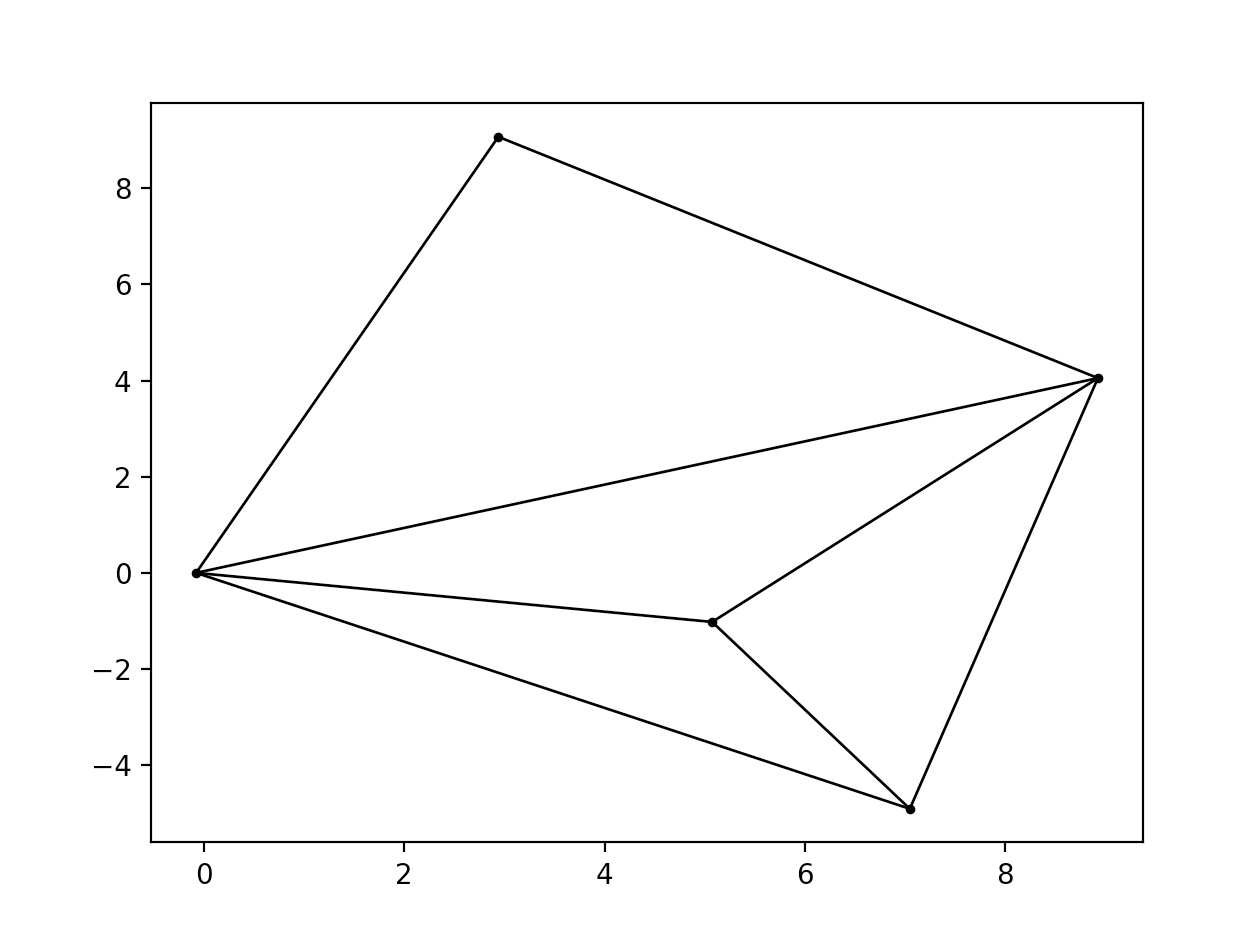
\includegraphics[width=70mm]{prim_h.png}
        \caption{Horizontal.}
    \end{minipage}\hfill
    \begin{minipage}{0.5\textwidth}
        \centering
        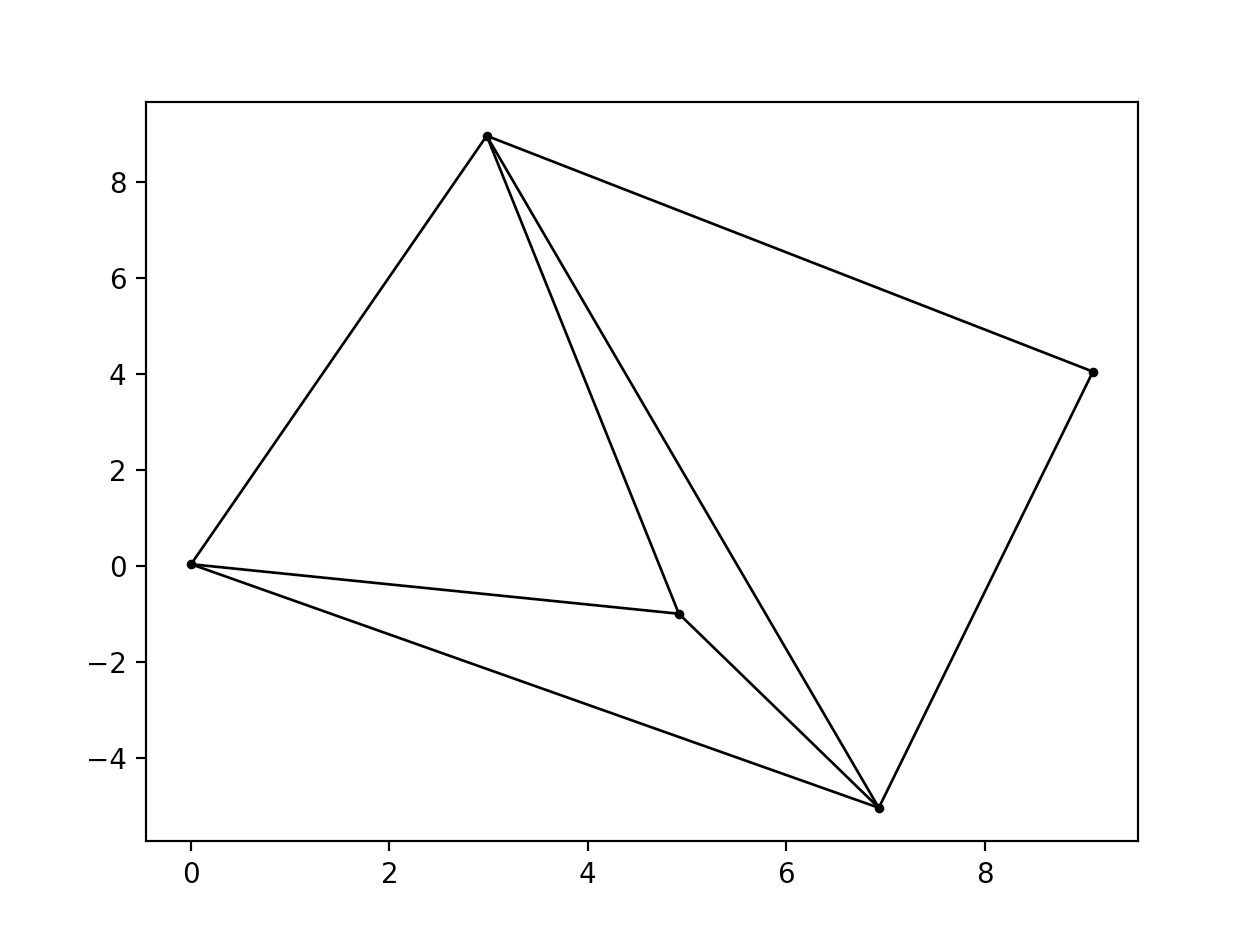
\includegraphics[width=70mm]{prim_v.png}
        \caption{Vertical.}
    \end{minipage}\hfill
\end{figure}

\noindent
\textbf{Example 2:} First example on 100 random points.
\begin{figure}[ht!]
    \centering
    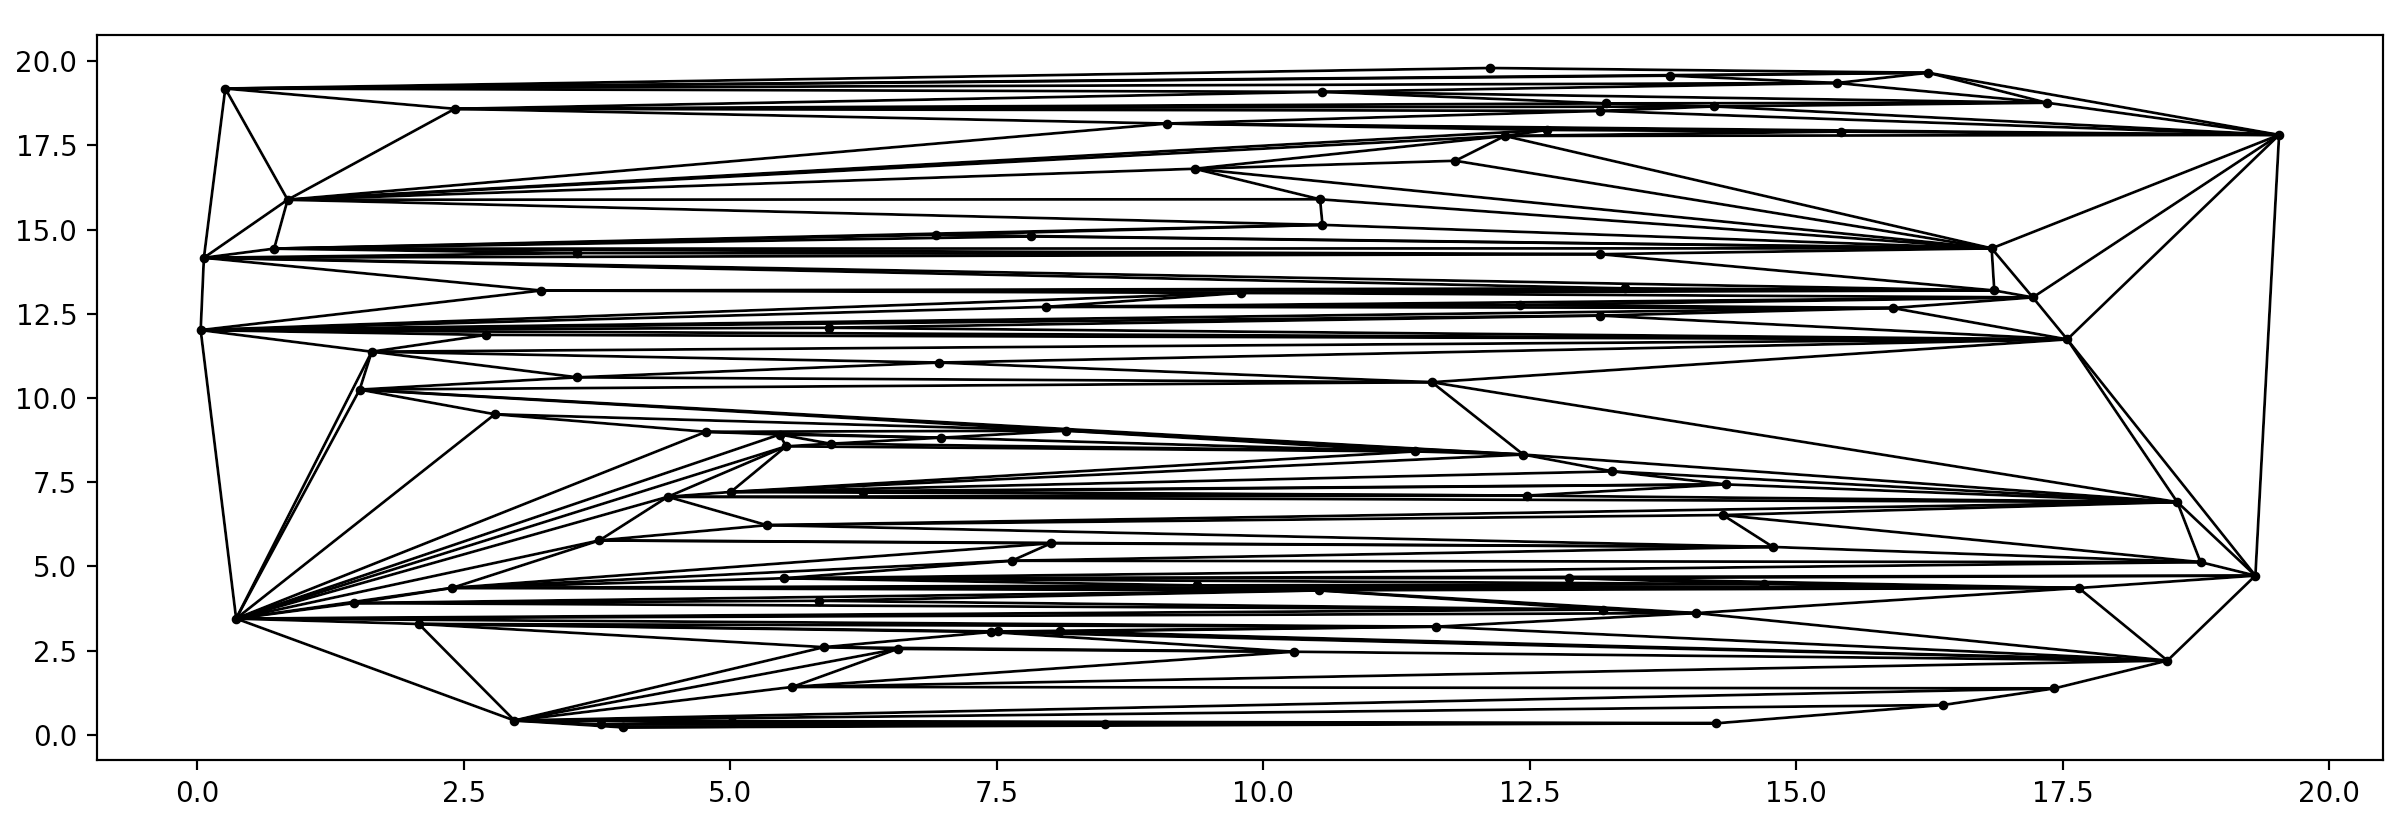
\includegraphics[width=150mm]{prim1_h.png}
    \caption{Horizontal.}
\end{figure}

\begin{figure}[ht!]
    \centering
    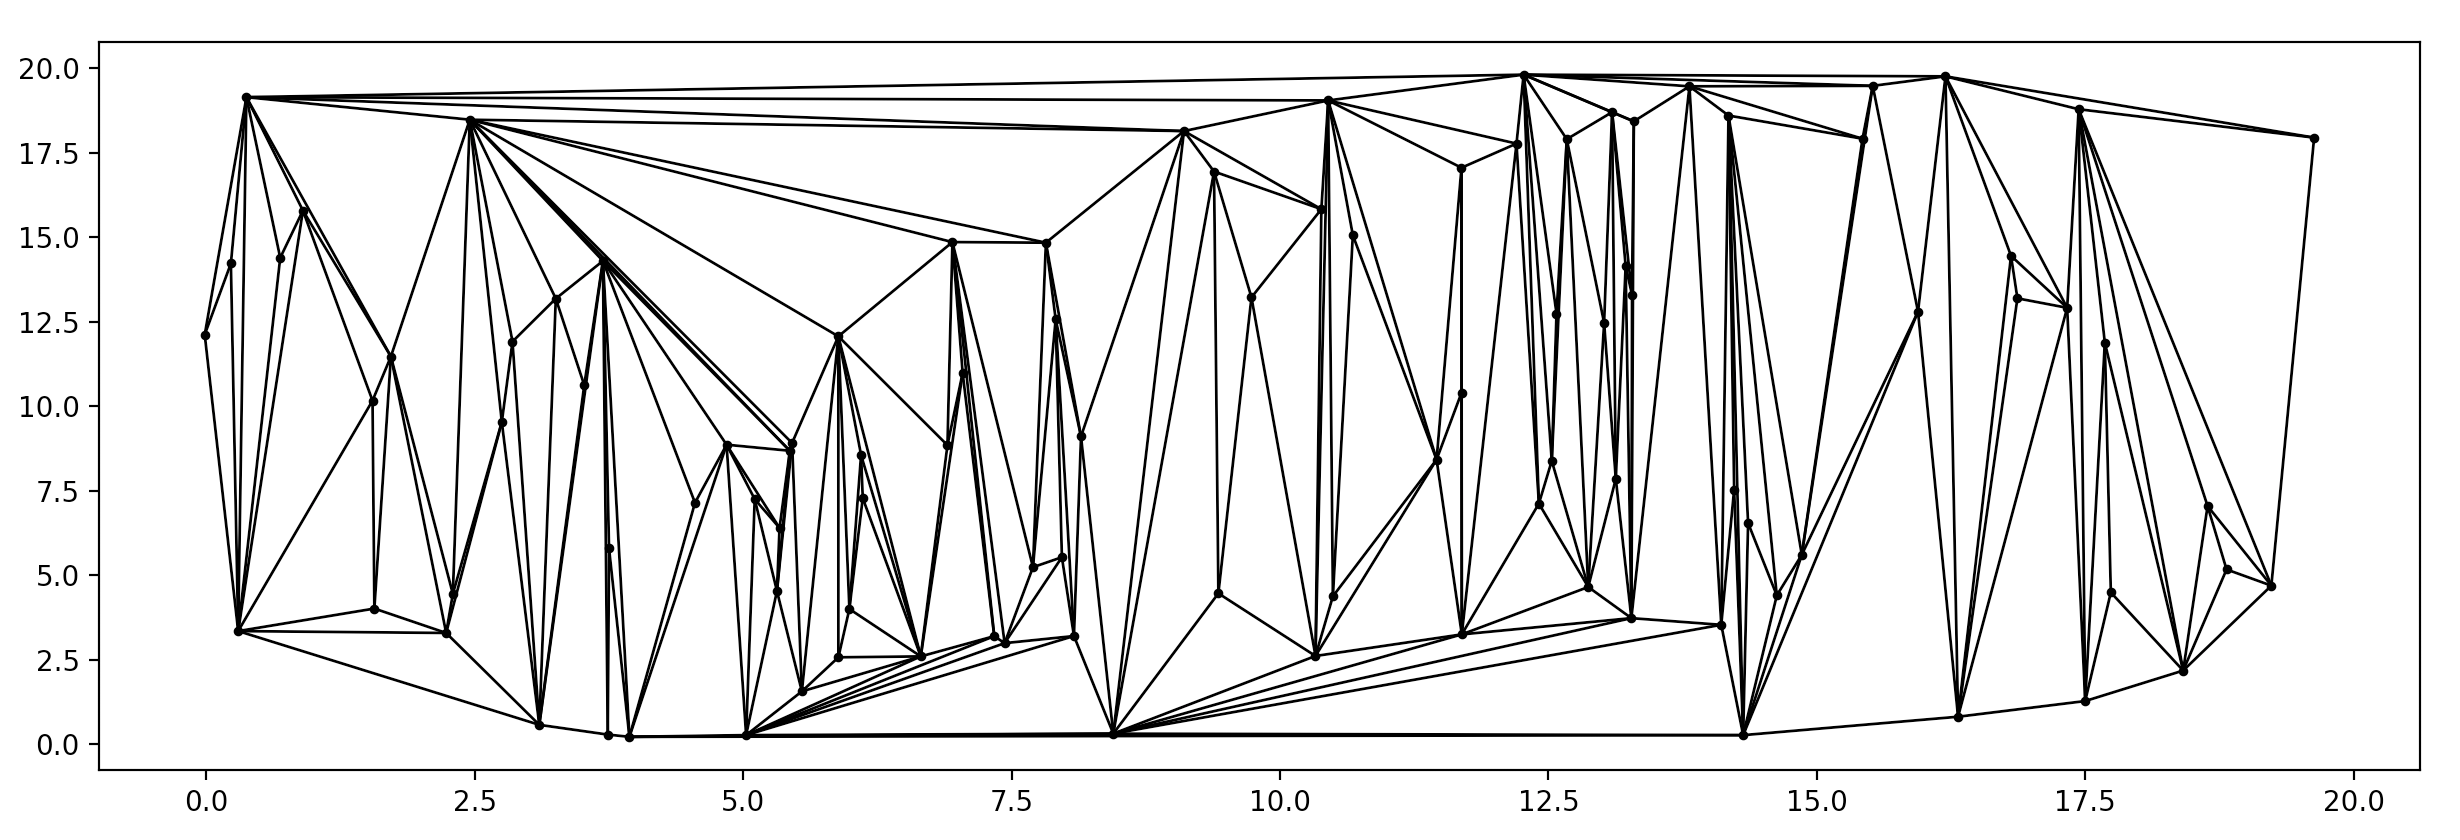
\includegraphics[width=150mm]{prim1_v.png}
    \caption{Vertical.}
\end{figure}

\newpage
\noindent
\textbf{Example 3:} Second example on 100 random points.
\begin{figure}[ht!]
    \centering
    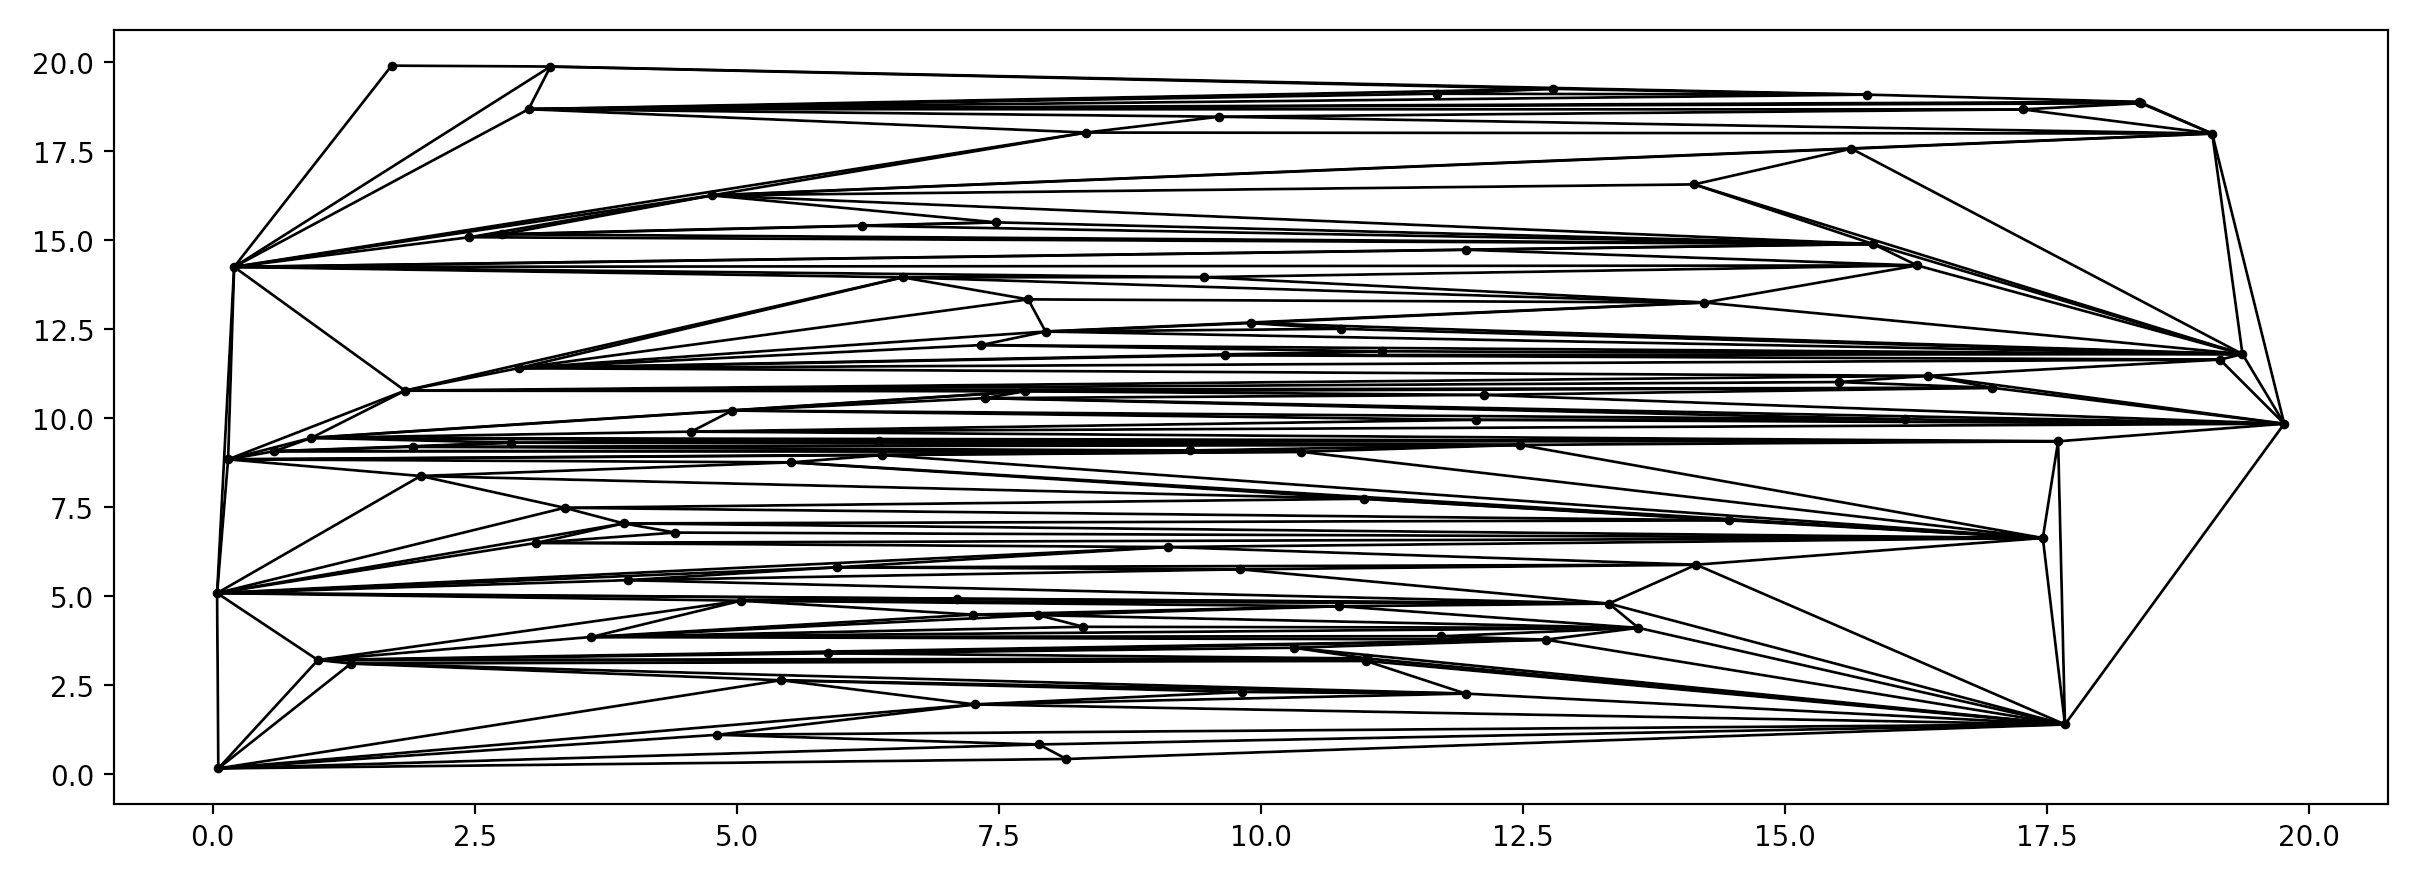
\includegraphics[width=150mm]{prim2_h.png}
    \caption{Horizontal.}
\end{figure}

\begin{figure}[ht!]
    \centering
    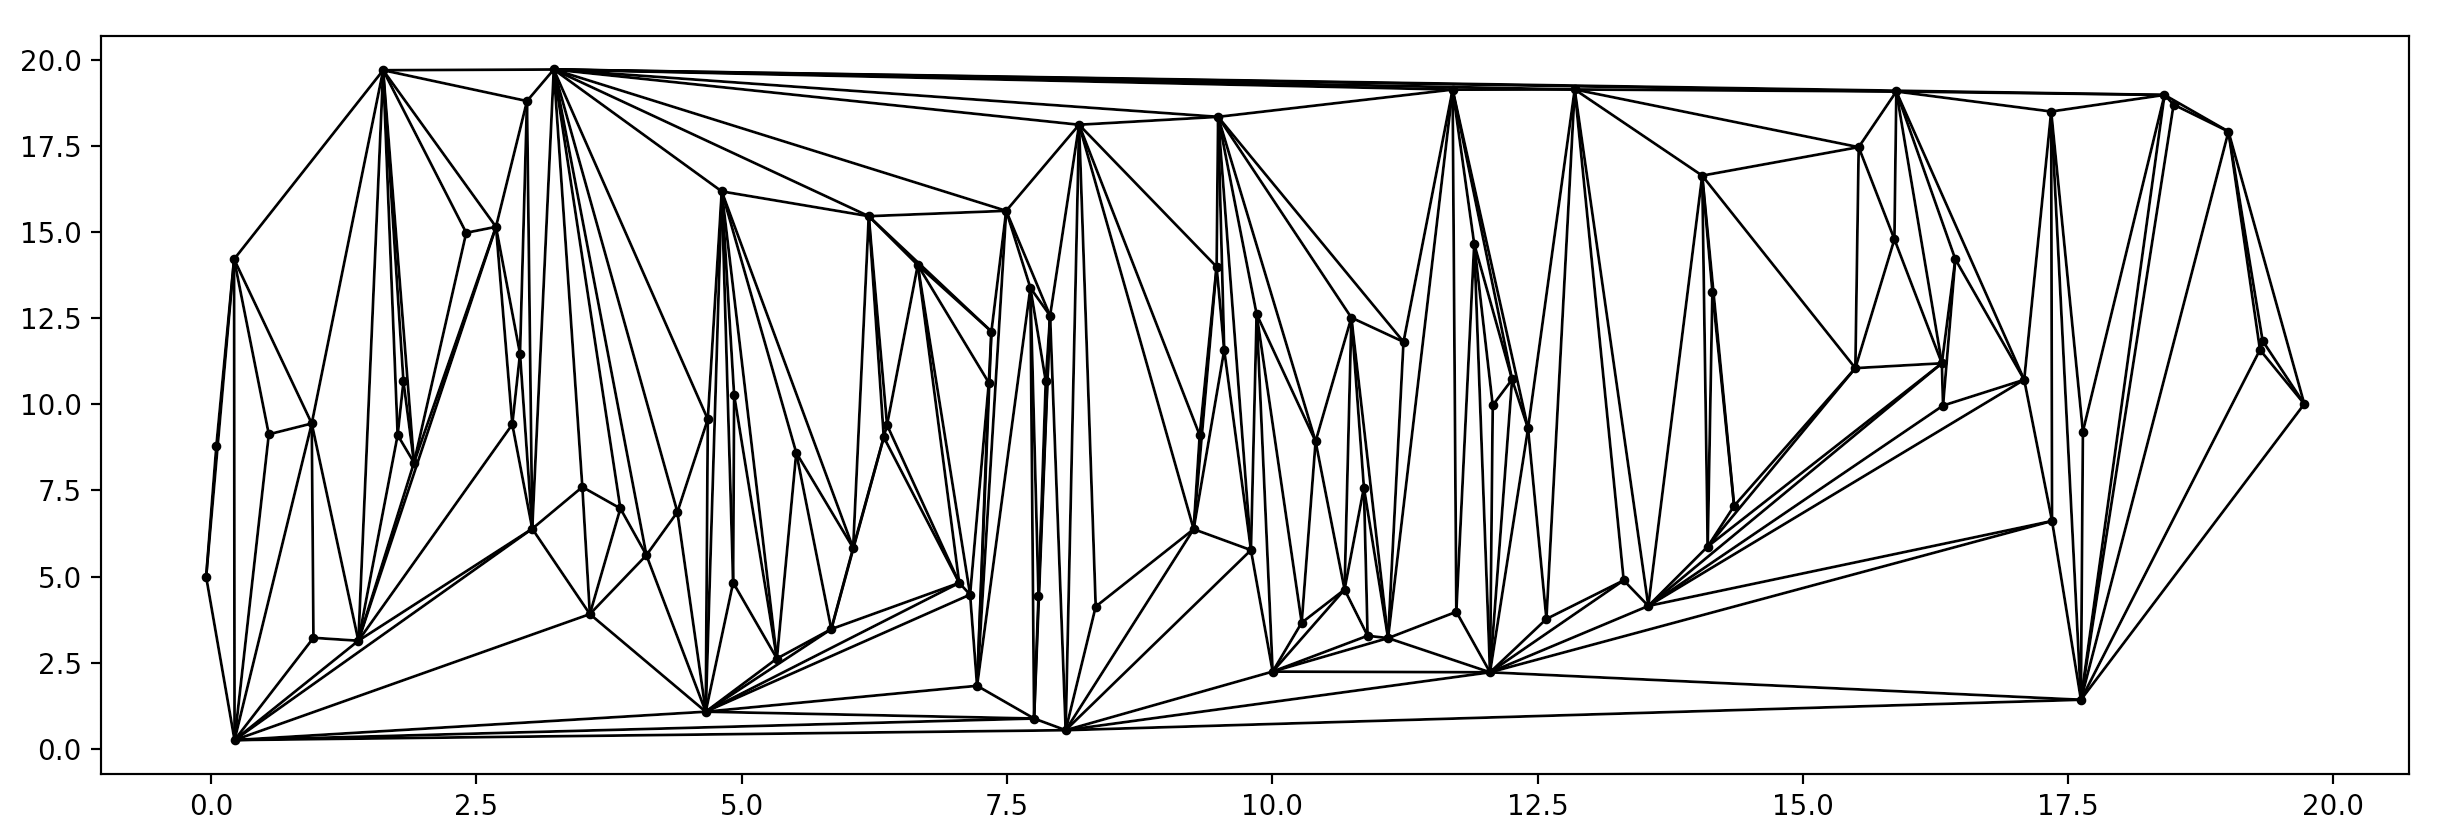
\includegraphics[width=150mm]{prim2_v.png}
    \caption{Vertical.}
\end{figure}

%%%%%%%%%%%%%%%%%%%%%%%%%%%%%%%%%%%%%%%%%%%%%%%%%%%%%%%%%%%%%%%%%%%%%%%%%%%%%%%%%%%%%%%%%%%%%%%%%%%%%%%%%%%%%%%%%%%%%%%%%%%%%%%%%%%%%%%%%%%%%%%%%%%%%%%%%%%%%%%%
\newpage
\subsection{Delauney triangulation}

Let $T$ be any triangulation. A function \texttt{optimize(T)} optimizes $T$ to produce the Delauney triangulation of the underlying set of points.
\\
All functions that we used are in the attached file \texttt{delauney.py}.
\\
First, the function makes a list of points in $T$ and then by using python library shapely makes a Delauney triangulation.
\\
\\
\textbf{Example 1:} Example from instructions.
\begin{figure}[ht!]
    \begin{minipage}{0.5\textwidth}
        \centering
        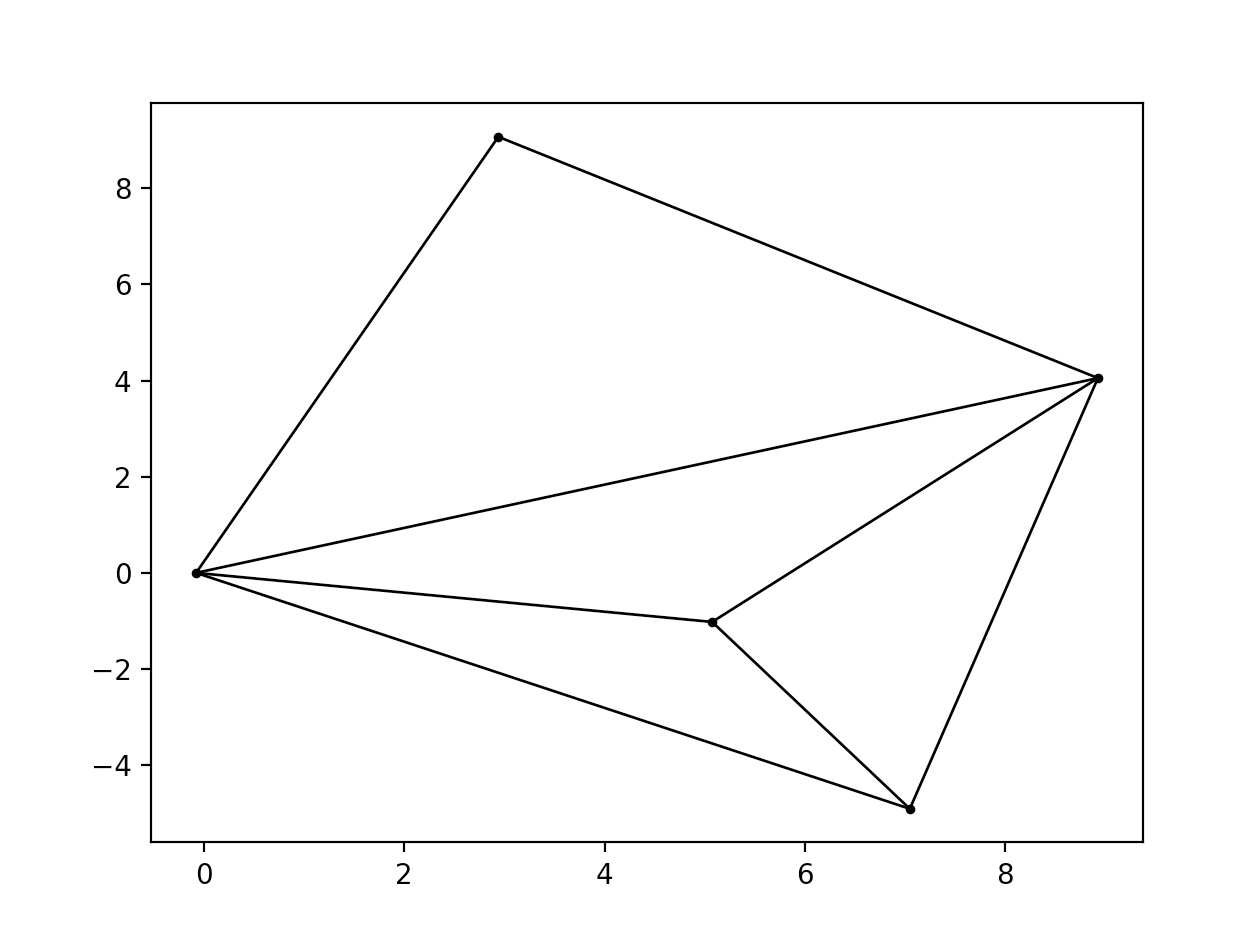
\includegraphics[width=70mm]{prim_h.png}
        \caption{Triangulation.}
    \end{minipage}\hfill
    \begin{minipage}{0.5\textwidth}
        \centering
        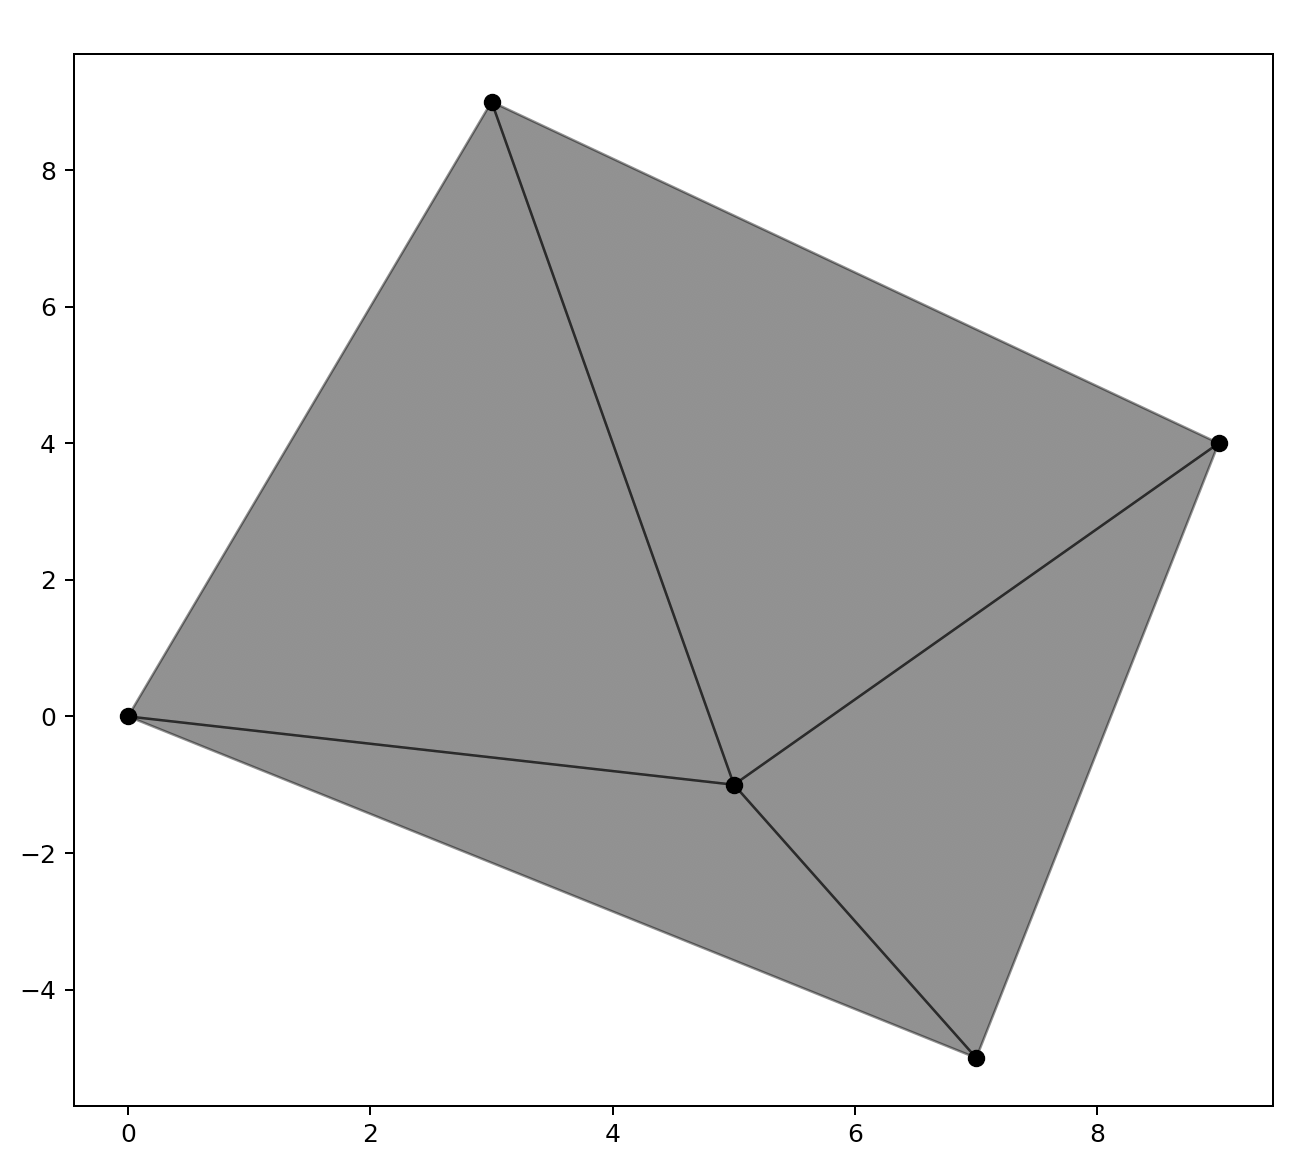
\includegraphics[width=50mm]{del.png}
        \caption{Delauney triangulation.}
    \end{minipage}\hfill
\end{figure}

\noindent
\textbf{Example 2:} First example on 100 random points.
\begin{figure}[ht!]
    \centering
    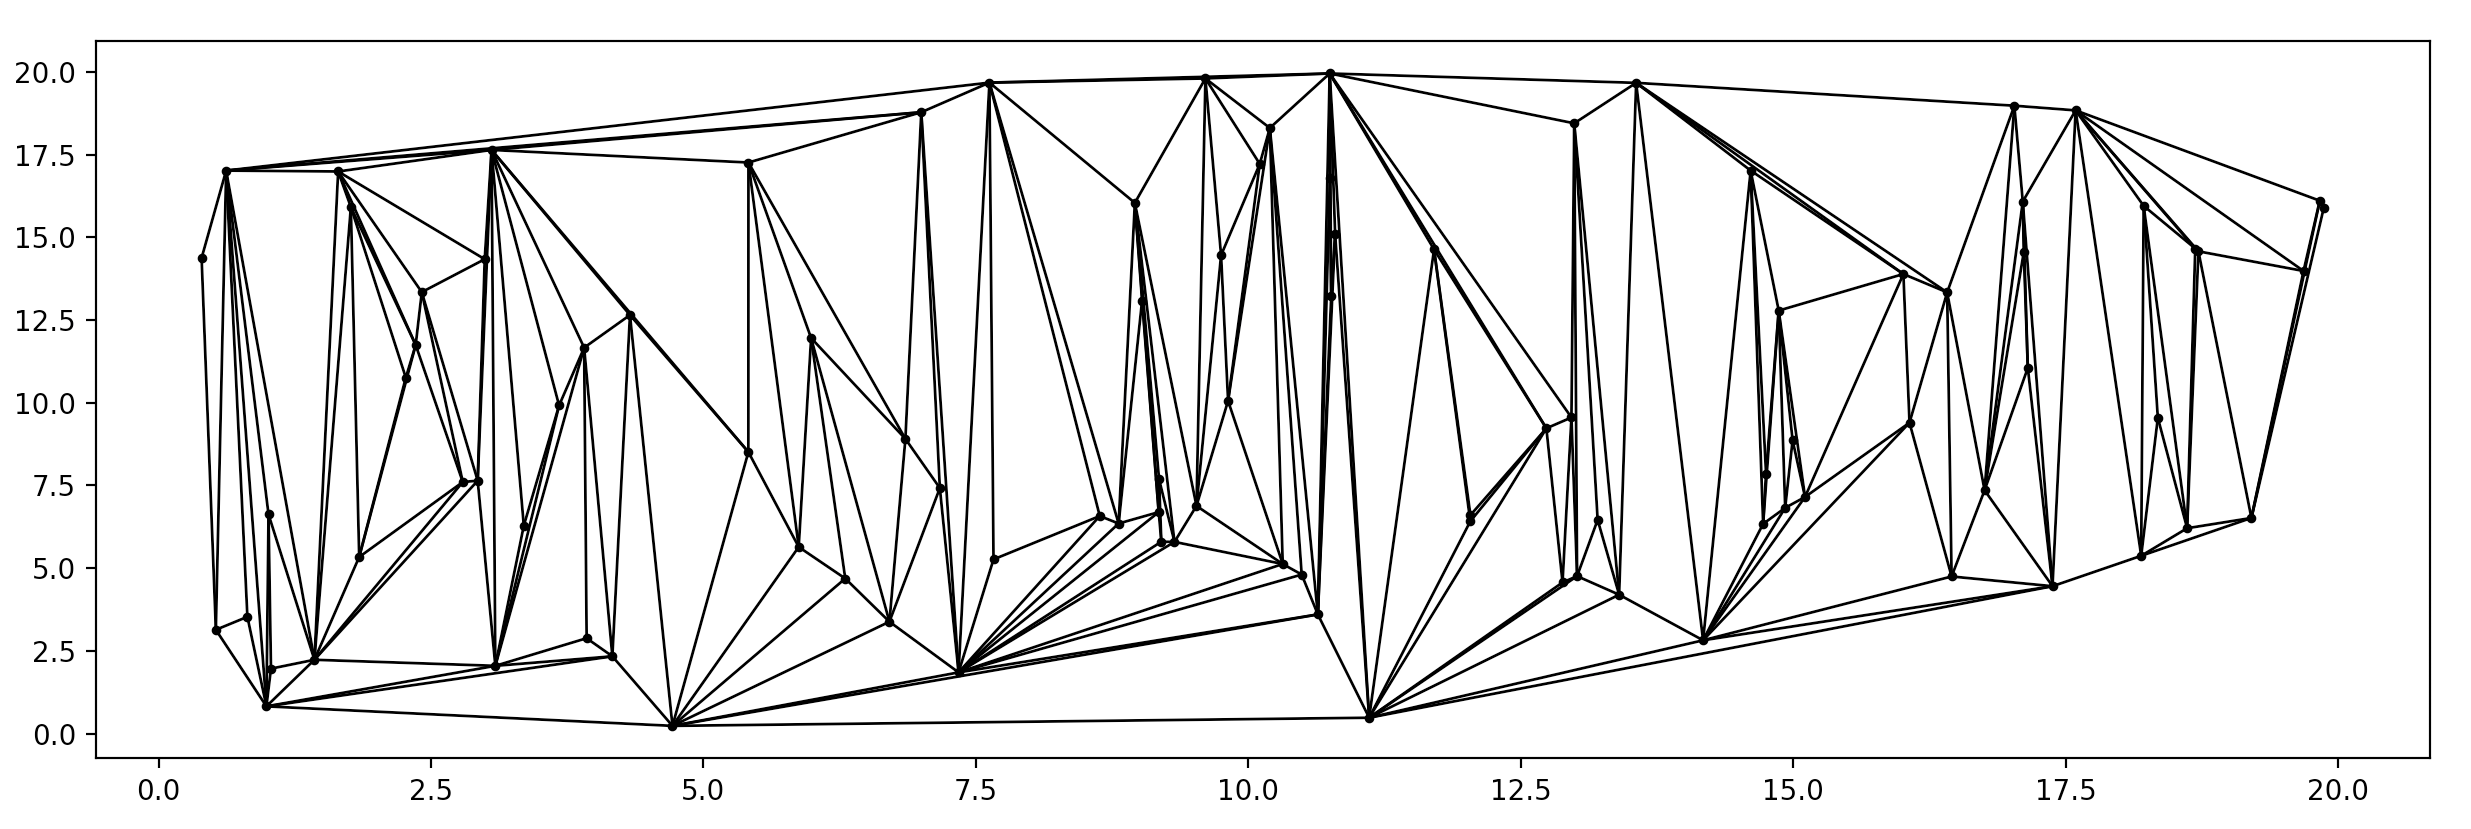
\includegraphics[width=150mm]{del_t1.png}
    \caption{Triangulation.}
\end{figure}
\begin{figure}[ht!]
    \centering
    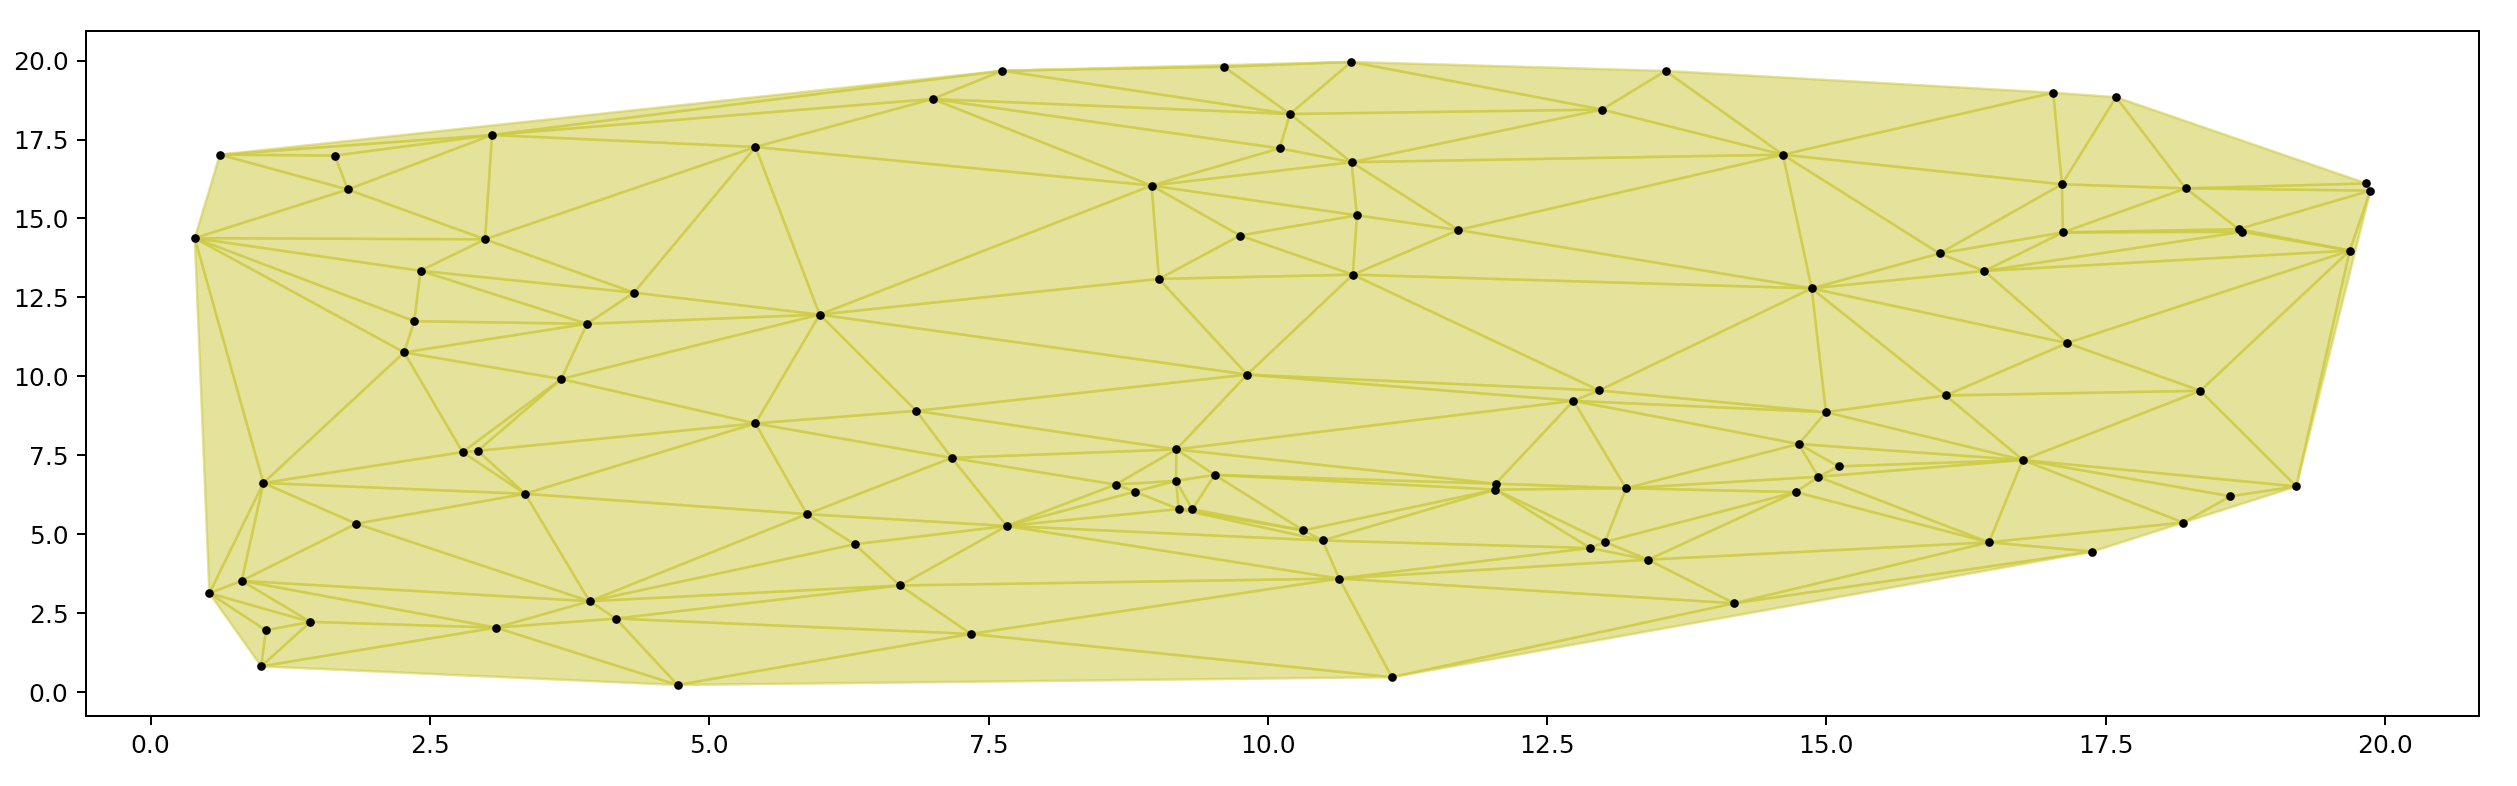
\includegraphics[width=150mm]{del_d1.png}
    \caption{Delauney triangulation.}
\end{figure}

\newpage
\noindent
\textbf{Example 3:} Second example on 100 random points.
\begin{figure}[ht!]
    \centering
    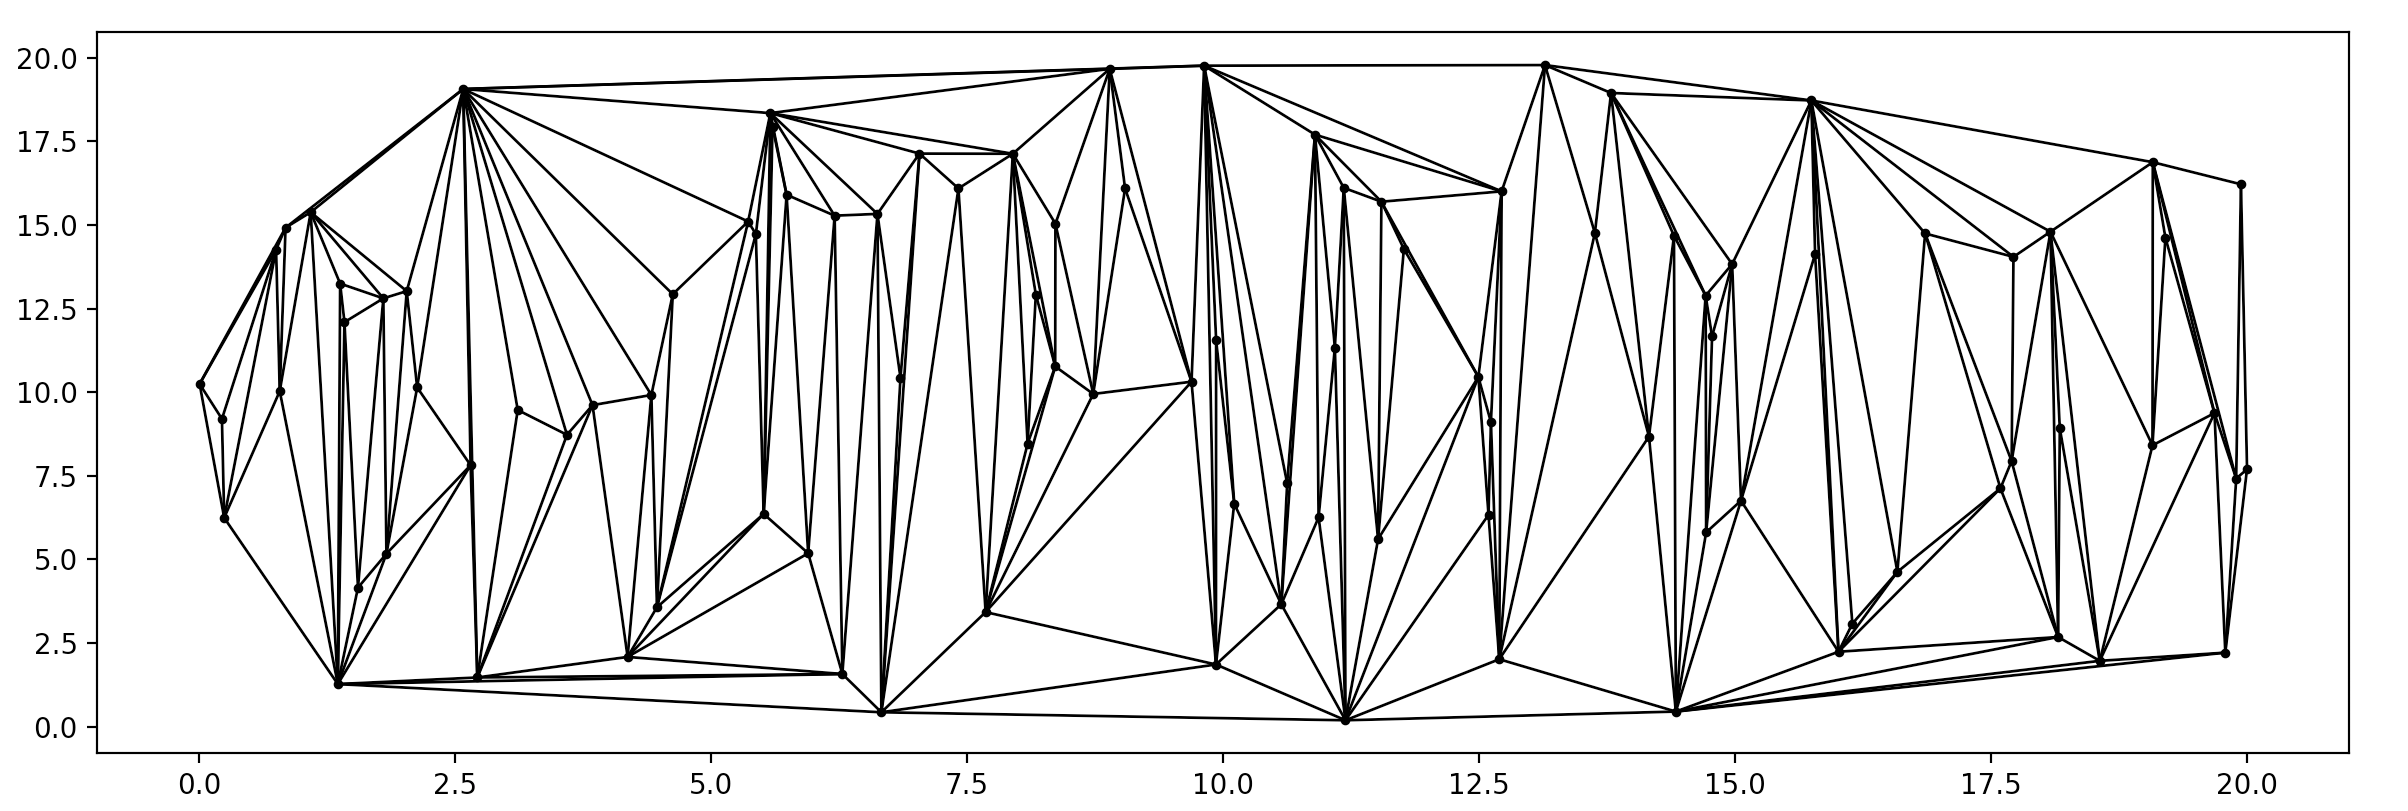
\includegraphics[width=150mm]{del_t2.png}
    \caption{Triangulation.}
\end{figure}
\begin{figure}[ht!]
    \centering
    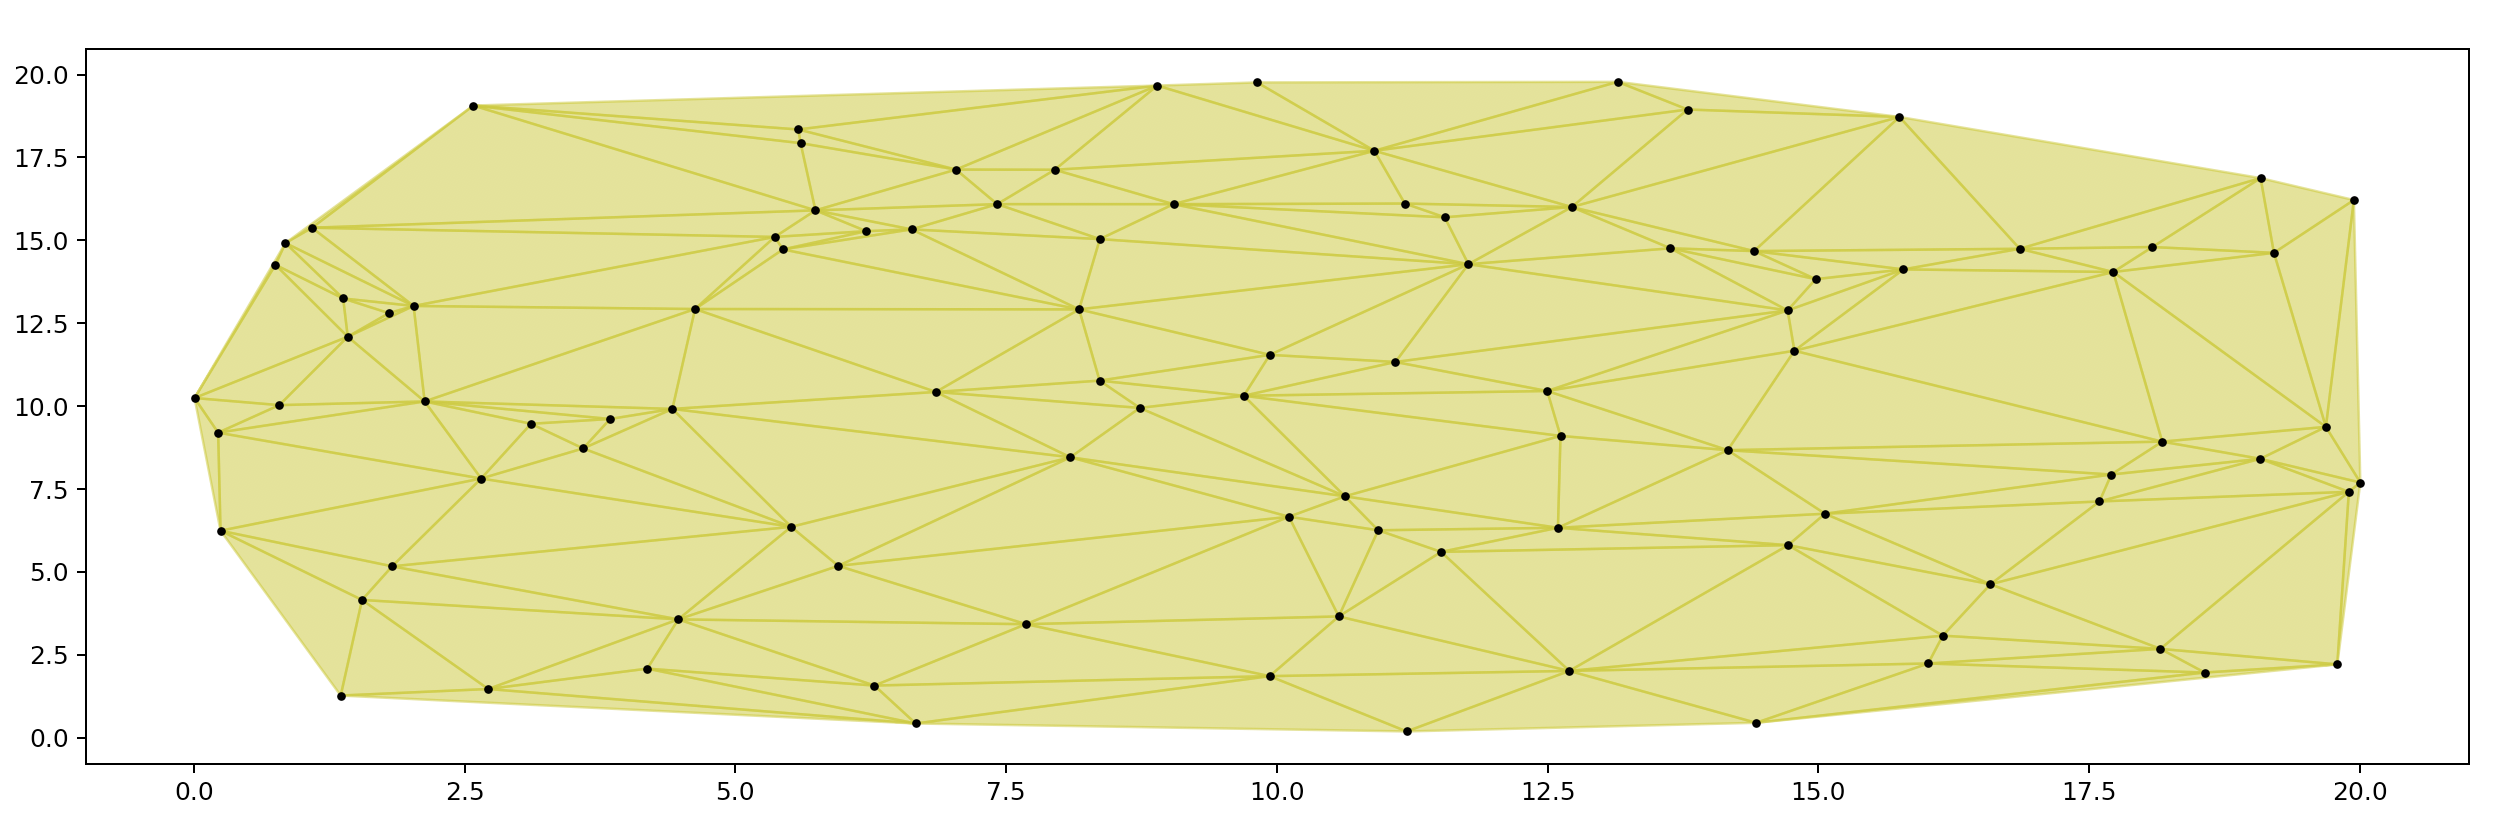
\includegraphics[width=150mm]{del_d2.png}
    \caption{Delauney triangulation.}
\end{figure}
%%%%%%%%%%%%%%%%%%%%%%%%%%%%%%%%%%%%%%%%%%%%%%%%%%%%%%%%%%%%%%%%%%%%%%%%%%%%%%%%%%%%%%%%%%%%%%%%%%%%%%%%%%%%%%%%%%%%%%%%%%%%%%%%%%%%%%%%%%%%%%%%%%%%%%%%%%%%%%%%

\newpage
\subsection{Orientation of surfaces}


%%%%%%%%%%%%%%%%%%%%%%%%%%%%%%%%%%%%%%%%%%%%%%%%%%%%%%%%%%%%%%%%%%%%%%%%%%%%%%%%%%%%%%%%%%%%%%%%%%%%%%%%%%%%%%%%%%%%%%%%%%%%%%%%%%%%%%%%%%%%%%%%%%%%%%%%%%%%%%%%

\end{document}